\documentclass{report}


%%%%%%%%%%%%%%%%%%%%%%%%%%%%%%%%%
% PACKAGE IMPORTS
%%%%%%%%%%%%%%%%%%%%%%%%%%%%%%%%%


\usepackage[tmargin=2cm,rmargin=1in,lmargin=1in,margin=0.85in,bmargin=2cm,footskip=.2in]{geometry}
\usepackage{amsmath,amsfonts,amsthm,amssymb,mathtools}
\usepackage[varbb]{newpxmath}
\usepackage{xfrac}
\usepackage[makeroom]{cancel}
\usepackage{mathtools}
\usepackage{bookmark}
\usepackage{enumitem}
\usepackage{hyperref,theoremref}
\usepackage{graphicx}
\graphicspath{ {./img} }
\hypersetup{
	pdftitle={Assignment},
	colorlinks=true, linkcolor=doc!90,
	bookmarksnumbered=true,
	bookmarksopen=true
}
\usepackage[most,many,breakable]{tcolorbox}
\usepackage{xcolor}
\usepackage{varwidth}
\usepackage{varwidth}
\usepackage{etoolbox}
%\usepackage{authblk}
\usepackage{nameref}
\usepackage{multicol,array}
\usepackage{tikz-cd}
\usepackage[ruled,vlined,linesnumbered]{algorithm2e}
\usepackage{comment} % enables the use of multi-line comments (\ifx \fi) 
\usepackage{import}
\usepackage{xifthen}
\usepackage{pdfpages}
\usepackage{transparent}

\newcommand\mycommfont[1]{\footnotesize\ttfamily\textcolor{blue}{#1}}
\SetCommentSty{mycommfont}
\newcommand{\incfig}[1]{%
    \def\svgwidth{\columnwidth}
    \import{./figures/}{#1.pdf_tex}
}

\usepackage{tikzsymbols}
\renewcommand\qedsymbol{$\Laughey$}


%\usepackage{import}
%\usepackage{xifthen}
%\usepackage{pdfpages}
%\usepackage{transparent}


%%%%%%%%%%%%%%%%%%%%%%%%%%%%%%
% SELF MADE COLORS
%%%%%%%%%%%%%%%%%%%%%%%%%%%%%%



\definecolor{myg}{RGB}{56, 140, 70}
\definecolor{myb}{RGB}{45, 111, 177}
\definecolor{myr}{RGB}{199, 68, 64}
\definecolor{mytheorembg}{HTML}{F2F2F9}
\definecolor{mytheoremfr}{HTML}{00007B}
\definecolor{mylenmabg}{HTML}{FFFAF8}
\definecolor{mylenmafr}{HTML}{983b0f}
\definecolor{mypropbg}{HTML}{f2fbfc}
\definecolor{mypropfr}{HTML}{191971}
\definecolor{myexamplebg}{HTML}{F2FBF8}
\definecolor{myexamplefr}{HTML}{88D6D1}
\definecolor{myexampleti}{HTML}{2A7F7F}
\definecolor{mydefinitbg}{HTML}{E5E5FF}
\definecolor{mydefinitfr}{HTML}{3F3FA3}
\definecolor{notesgreen}{RGB}{0,162,0}
\definecolor{myp}{RGB}{197, 92, 212}
\definecolor{mygr}{HTML}{2C3338}
\definecolor{myred}{RGB}{127,0,0}
\definecolor{myyellow}{RGB}{169,121,69}
\definecolor{myexercisebg}{HTML}{F2FBF8}
\definecolor{myexercisefg}{HTML}{88D6D1}


%%%%%%%%%%%%%%%%%%%%%%%%%%%%
% TCOLORBOX SETUPS
%%%%%%%%%%%%%%%%%%%%%%%%%%%%

\setlength{\parindent}{1cm}
%================================
% THEOREM BOX
%================================

\tcbuselibrary{theorems,skins,hooks}
\newtcbtheorem[number within=section]{Theorem}{Theorem}
{%
	enhanced,
	breakable,
	colback = mytheorembg,
	frame hidden,
	boxrule = 0sp,
	borderline west = {2pt}{0pt}{mytheoremfr},
	sharp corners,
	detach title,
	before upper = \tcbtitle\par\smallskip,
	coltitle = mytheoremfr,
	fonttitle = \bfseries\sffamily,
	description font = \mdseries,
	separator sign none,
	segmentation style={solid, mytheoremfr},
}
{th}

\tcbuselibrary{theorems,skins,hooks}
\newtcbtheorem[number within=chapter]{theorem}{Theorem}
{%
	enhanced,
	breakable,
	colback = mytheorembg,
	frame hidden,
	boxrule = 0sp,
	borderline west = {2pt}{0pt}{mytheoremfr},
	sharp corners,
	detach title,
	before upper = \tcbtitle\par\smallskip,
	coltitle = mytheoremfr,
	fonttitle = \bfseries\sffamily,
	description font = \mdseries,
	separator sign none,
	segmentation style={solid, mytheoremfr},
}
{th}


\tcbuselibrary{theorems,skins,hooks}
\newtcolorbox{Theoremcon}
{%
	enhanced
	,breakable
	,colback = mytheorembg
	,frame hidden
	,boxrule = 0sp
	,borderline west = {2pt}{0pt}{mytheoremfr}
	,sharp corners
	,description font = \mdseries
	,separator sign none
}

%================================
% Corollery
%================================
\tcbuselibrary{theorems,skins,hooks}
\newtcbtheorem[number within=section]{Corollary}{Corollary}
{%
	enhanced
	,breakable
	,colback = myp!10
	,frame hidden
	,boxrule = 0sp
	,borderline west = {2pt}{0pt}{myp!85!black}
	,sharp corners
	,detach title
	,before upper = \tcbtitle\par\smallskip
	,coltitle = myp!85!black
	,fonttitle = \bfseries\sffamily
	,description font = \mdseries
	,separator sign none
	,segmentation style={solid, myp!85!black}
}
{th}
\tcbuselibrary{theorems,skins,hooks}
\newtcbtheorem[number within=chapter]{corollary}{Corollary}
{%
	enhanced
	,breakable
	,colback = myp!10
	,frame hidden
	,boxrule = 0sp
	,borderline west = {2pt}{0pt}{myp!85!black}
	,sharp corners
	,detach title
	,before upper = \tcbtitle\par\smallskip
	,coltitle = myp!85!black
	,fonttitle = \bfseries\sffamily
	,description font = \mdseries
	,separator sign none
	,segmentation style={solid, myp!85!black}
}
{th}


%================================
% LENMA
%================================

\tcbuselibrary{theorems,skins,hooks}
\newtcbtheorem[number within=section]{Lenma}{Lenma}
{%
	enhanced,
	breakable,
	colback = mylenmabg,
	frame hidden,
	boxrule = 0sp,
	borderline west = {2pt}{0pt}{mylenmafr},
	sharp corners,
	detach title,
	before upper = \tcbtitle\par\smallskip,
	coltitle = mylenmafr,
	fonttitle = \bfseries\sffamily,
	description font = \mdseries,
	separator sign none,
	segmentation style={solid, mylenmafr},
}
{th}

\tcbuselibrary{theorems,skins,hooks}
\newtcbtheorem[number within=chapter]{lenma}{Lenma}
{%
	enhanced,
	breakable,
	colback = mylenmabg,
	frame hidden,
	boxrule = 0sp,
	borderline west = {2pt}{0pt}{mylenmafr},
	sharp corners,
	detach title,
	before upper = \tcbtitle\par\smallskip,
	coltitle = mylenmafr,
	fonttitle = \bfseries\sffamily,
	description font = \mdseries,
	separator sign none,
	segmentation style={solid, mylenmafr},
}
{th}


%================================
% PROPOSITION
%================================

\tcbuselibrary{theorems,skins,hooks}
\newtcbtheorem[number within=section]{Prop}{Proposition}
{%
	enhanced,
	breakable,
	colback = mypropbg,
	frame hidden,
	boxrule = 0sp,
	borderline west = {2pt}{0pt}{mypropfr},
	sharp corners,
	detach title,
	before upper = \tcbtitle\par\smallskip,
	coltitle = mypropfr,
	fonttitle = \bfseries\sffamily,
	description font = \mdseries,
	separator sign none,
	segmentation style={solid, mypropfr},
}
{th}

\tcbuselibrary{theorems,skins,hooks}
\newtcbtheorem[number within=chapter]{prop}{Proposition}
{%
	enhanced,
	breakable,
	colback = mypropbg,
	frame hidden,
	boxrule = 0sp,
	borderline west = {2pt}{0pt}{mypropfr},
	sharp corners,
	detach title,
	before upper = \tcbtitle\par\smallskip,
	coltitle = mypropfr,
	fonttitle = \bfseries\sffamily,
	description font = \mdseries,
	separator sign none,
	segmentation style={solid, mypropfr},
}
{th}


%================================
% CLAIM
%================================

\tcbuselibrary{theorems,skins,hooks}
\newtcbtheorem[number within=section]{claim}{Claim}
{%
	enhanced
	,breakable
	,colback = myg!10
	,frame hidden
	,boxrule = 0sp
	,borderline west = {2pt}{0pt}{myg}
	,sharp corners
	,detach title
	,before upper = \tcbtitle\par\smallskip
	,coltitle = myg!85!black
	,fonttitle = \bfseries\sffamily
	,description font = \mdseries
	,separator sign none
	,segmentation style={solid, myg!85!black}
}
{th}



%================================
% Exercise
%================================

\tcbuselibrary{theorems,skins,hooks}
\newtcbtheorem[number within=section]{Exercise}{Exercise}
{%
	enhanced,
	breakable,
	colback = myexercisebg,
	frame hidden,
	boxrule = 0sp,
	borderline west = {2pt}{0pt}{myexercisefg},
	sharp corners,
	detach title,
	before upper = \tcbtitle\par\smallskip,
	coltitle = myexercisefg,
	fonttitle = \bfseries\sffamily,
	description font = \mdseries,
	separator sign none,
	segmentation style={solid, myexercisefg},
}
{th}

\tcbuselibrary{theorems,skins,hooks}
\newtcbtheorem[number within=chapter]{exercise}{Exercise}
{%
	enhanced,
	breakable,
	colback = myexercisebg,
	frame hidden,
	boxrule = 0sp,
	borderline west = {2pt}{0pt}{myexercisefg},
	sharp corners,
	detach title,
	before upper = \tcbtitle\par\smallskip,
	coltitle = myexercisefg,
	fonttitle = \bfseries\sffamily,
	description font = \mdseries,
	separator sign none,
	segmentation style={solid, myexercisefg},
}
{th}

%================================
% EXAMPLE BOX
%================================

\newtcbtheorem[number within=section]{Example}{Example}
{%
	colback = myexamplebg
	,breakable
	,colframe = myexamplefr
	,coltitle = myexampleti
	,boxrule = 1pt
	,sharp corners
	,detach title
	,before upper=\tcbtitle\par\smallskip
	,fonttitle = \bfseries
	,description font = \mdseries
	,separator sign none
	,description delimiters parenthesis
}
{ex}

\newtcbtheorem[number within=chapter]{example}{Example}
{%
	colback = myexamplebg
	,breakable
	,colframe = myexamplefr
	,coltitle = myexampleti
	,boxrule = 1pt
	,sharp corners
	,detach title
	,before upper=\tcbtitle\par\smallskip
	,fonttitle = \bfseries
	,description font = \mdseries
	,separator sign none
	,description delimiters parenthesis
}
{ex}

%================================
% DEFINITION BOX
%================================

\newtcbtheorem[number within=section]{Definition}{Definition}{enhanced,
	before skip=2mm,after skip=2mm, colback=red!5,colframe=red!80!black,boxrule=0.5mm,
	attach boxed title to top left={xshift=1cm,yshift*=1mm-\tcboxedtitleheight}, varwidth boxed title*=-3cm,
	boxed title style={frame code={
					\path[fill=tcbcolback]
					([yshift=-1mm,xshift=-1mm]frame.north west)
					arc[start angle=0,end angle=180,radius=1mm]
					([yshift=-1mm,xshift=1mm]frame.north east)
					arc[start angle=180,end angle=0,radius=1mm];
					\path[left color=tcbcolback!60!black,right color=tcbcolback!60!black,
						middle color=tcbcolback!80!black]
					([xshift=-2mm]frame.north west) -- ([xshift=2mm]frame.north east)
					[rounded corners=1mm]-- ([xshift=1mm,yshift=-1mm]frame.north east)
					-- (frame.south east) -- (frame.south west)
					-- ([xshift=-1mm,yshift=-1mm]frame.north west)
					[sharp corners]-- cycle;
				},interior engine=empty,
		},
	fonttitle=\bfseries,
	title={#2},#1}{def}
\newtcbtheorem[number within=chapter]{definition}{Definition}{enhanced,
	before skip=2mm,after skip=2mm, colback=red!5,colframe=red!80!black,boxrule=0.5mm,
	attach boxed title to top left={xshift=1cm,yshift*=1mm-\tcboxedtitleheight}, varwidth boxed title*=-3cm,
	boxed title style={frame code={
					\path[fill=tcbcolback]
					([yshift=-1mm,xshift=-1mm]frame.north west)
					arc[start angle=0,end angle=180,radius=1mm]
					([yshift=-1mm,xshift=1mm]frame.north east)
					arc[start angle=180,end angle=0,radius=1mm];
					\path[left color=tcbcolback!60!black,right color=tcbcolback!60!black,
						middle color=tcbcolback!80!black]
					([xshift=-2mm]frame.north west) -- ([xshift=2mm]frame.north east)
					[rounded corners=1mm]-- ([xshift=1mm,yshift=-1mm]frame.north east)
					-- (frame.south east) -- (frame.south west)
					-- ([xshift=-1mm,yshift=-1mm]frame.north west)
					[sharp corners]-- cycle;
				},interior engine=empty,
		},
	fonttitle=\bfseries,
	title={#2},#1}{def}



%================================
% Solution BOX
%================================

\makeatletter
\newtcbtheorem{question}{Question}{enhanced,
	breakable,
	colback=white,
	colframe=myb!80!black,
	attach boxed title to top left={yshift*=-\tcboxedtitleheight},
	fonttitle=\bfseries,
	title={#2},
	boxed title size=title,
	boxed title style={%
			sharp corners,
			rounded corners=northwest,
			colback=tcbcolframe,
			boxrule=0pt,
		},
	underlay boxed title={%
			\path[fill=tcbcolframe] (title.south west)--(title.south east)
			to[out=0, in=180] ([xshift=5mm]title.east)--
			(title.center-|frame.east)
			[rounded corners=\kvtcb@arc] |-
			(frame.north) -| cycle;
		},
	#1
}{def}
\makeatother

%================================
% SOLUTION BOX
%================================

\makeatletter
\newtcolorbox{solution}{enhanced,
	breakable,
	colback=white,
	colframe=myg!80!black,
	attach boxed title to top left={yshift*=-\tcboxedtitleheight},
	title=Solution,
	boxed title size=title,
	boxed title style={%
			sharp corners,
			rounded corners=northwest,
			colback=tcbcolframe,
			boxrule=0pt,
		},
	underlay boxed title={%
			\path[fill=tcbcolframe] (title.south west)--(title.south east)
			to[out=0, in=180] ([xshift=5mm]title.east)--
			(title.center-|frame.east)
			[rounded corners=\kvtcb@arc] |-
			(frame.north) -| cycle;
		},
}
\makeatother

%================================
% Question BOX
%================================

\makeatletter
\newtcbtheorem{qstion}{Question}{enhanced,
	breakable,
	colback=white,
	colframe=mygr,
	attach boxed title to top left={yshift*=-\tcboxedtitleheight},
	fonttitle=\bfseries,
	title={#2},
	boxed title size=title,
	boxed title style={%
			sharp corners,
			rounded corners=northwest,
			colback=tcbcolframe,
			boxrule=0pt,
		},
	underlay boxed title={%
			\path[fill=tcbcolframe] (title.south west)--(title.south east)
			to[out=0, in=180] ([xshift=5mm]title.east)--
			(title.center-|frame.east)
			[rounded corners=\kvtcb@arc] |-
			(frame.north) -| cycle;
		},
	#1
}{def}
\makeatother

\newtcbtheorem[number within=chapter]{wconc}{Wrong Concept}{
	breakable,
	enhanced,
	colback=white,
	colframe=myr,
	arc=0pt,
	outer arc=0pt,
	fonttitle=\bfseries\sffamily\large,
	colbacktitle=myr,
	attach boxed title to top left={},
	boxed title style={
			enhanced,
			skin=enhancedfirst jigsaw,
			arc=3pt,
			bottom=0pt,
			interior style={fill=myr}
		},
	#1
}{def}



%================================
% NOTE BOX
%================================

\usetikzlibrary{arrows,calc,shadows.blur}
\tcbuselibrary{skins}
\newtcolorbox{note}[1][]{%
	enhanced jigsaw,
	colback=gray!20!white,%
	colframe=gray!80!black,
	size=small,
	boxrule=1pt,
	title=\textbf{Note:-},
	halign title=flush center,
	coltitle=black,
	breakable,
	drop shadow=black!50!white,
	attach boxed title to top left={xshift=1cm,yshift=-\tcboxedtitleheight/2,yshifttext=-\tcboxedtitleheight/2},
	minipage boxed title=1.5cm,
	boxed title style={%
			colback=white,
			size=fbox,
			boxrule=1pt,
			boxsep=2pt,
			underlay={%
					\coordinate (dotA) at ($(interior.west) + (-0.5pt,0)$);
					\coordinate (dotB) at ($(interior.east) + (0.5pt,0)$);
					\begin{scope}
						\clip (interior.north west) rectangle ([xshift=3ex]interior.east);
						\filldraw [white, blur shadow={shadow opacity=60, shadow yshift=-.75ex}, rounded corners=2pt] (interior.north west) rectangle (interior.south east);
					\end{scope}
					\begin{scope}[gray!80!black]
						\fill (dotA) circle (2pt);
						\fill (dotB) circle (2pt);
					\end{scope}
				},
		},
	#1,
}

%%%%%%%%%%%%%%%%%%%%%%%%%%%%%%
% SELF MADE COMMANDS
%%%%%%%%%%%%%%%%%%%%%%%%%%%%%%


\newcommand{\thm}[2]{\begin{Theorem}{#1}{}#2\end{Theorem}}
\newcommand{\cor}[2]{\begin{Corollary}{#1}{}#2\end{Corollary}}
\newcommand{\mlenma}[2]{\begin{Lenma}{#1}{}#2\end{Lenma}}
\newcommand{\mprop}[2]{\begin{Prop}{#1}{}#2\end{Prop}}
\newcommand{\clm}[3]{\begin{claim}{#1}{#2}#3\end{claim}}
\newcommand{\wc}[2]{\begin{wconc}{#1}{}\setlength{\parindent}{1cm}#2\end{wconc}}
\newcommand{\thmcon}[1]{\begin{Theoremcon}{#1}\end{Theoremcon}}
\newcommand{\ex}[2]{\begin{Example}{#1}{}#2\end{Example}}
\newcommand{\dfn}[2]{\begin{Definition}[colbacktitle=red!75!black]{#1}{}#2\end{Definition}}
\newcommand{\dfnc}[2]{\begin{definition}[colbacktitle=red!75!black]{#1}{}#2\end{definition}}
\newcommand{\qs}[2]{\begin{question}{#1}{}#2\end{question}}
\newcommand{\pf}[2]{\begin{myproof}[#1]#2\end{myproof}}
\newcommand{\nt}[1]{\begin{note}#1\end{note}}

\newcommand*\circled[1]{\tikz[baseline=(char.base)]{
		\node[shape=circle,draw,inner sep=1pt] (char) {#1};}}
\newcommand\getcurrentref[1]{%
	\ifnumequal{\value{#1}}{0}
	{??}
	{\the\value{#1}}%
}
\newcommand{\getCurrentSectionNumber}{\getcurrentref{section}}
\newenvironment{myproof}[1][\proofname]{%
	\proof[\bfseries #1: ]%
}{\endproof}

\newcommand{\mclm}[2]{\begin{myclaim}[#1]#2\end{myclaim}}
\newenvironment{myclaim}[1][\claimname]{\proof[\bfseries #1: ]}{}

\newcounter{mylabelcounter}

\makeatletter
\newcommand{\setword}[2]{%
	\phantomsection
	#1\def\@currentlabel{\unexpanded{#1}}\label{#2}%
}
\makeatother




\tikzset{
	symbol/.style={
			draw=none,
			every to/.append style={
					edge node={node [sloped, allow upside down, auto=false]{$#1$}}}
		}
}


% deliminators
\DeclarePairedDelimiter{\abs}{\lvert}{\rvert}
\DeclarePairedDelimiter{\norm}{\lVert}{\rVert}

\DeclarePairedDelimiter{\ceil}{\lceil}{\rceil}
\DeclarePairedDelimiter{\floor}{\lfloor}{\rfloor}
\DeclarePairedDelimiter{\round}{\lfloor}{\rceil}

\newsavebox\diffdbox
\newcommand{\slantedromand}{{\mathpalette\makesl{d}}}
\newcommand{\makesl}[2]{%
\begingroup
\sbox{\diffdbox}{$\mathsurround=0pt#1\mathrm{#2}$}%
\pdfsave
\pdfsetmatrix{1 0 0.2 1}%
\rlap{\usebox{\diffdbox}}%
\pdfrestore
\hskip\wd\diffdbox
\endgroup
}
\newcommand{\dd}[1][]{\ensuremath{\mathop{}\!\ifstrempty{#1}{%
\slantedromand\@ifnextchar^{\hspace{0.2ex}}{\hspace{0.1ex}}}%
{\slantedromand\hspace{0.2ex}^{#1}}}}
\ProvideDocumentCommand\dv{o m g}{%
  \ensuremath{%
    \IfValueTF{#3}{%
      \IfNoValueTF{#1}{%
        \frac{\dd #2}{\dd #3}%
      }{%
        \frac{\dd^{#1} #2}{\dd #3^{#1}}%
      }%
    }{%
      \IfNoValueTF{#1}{%
        \frac{\dd}{\dd #2}%
      }{%
        \frac{\dd^{#1}}{\dd #2^{#1}}%
      }%
    }%
  }%
}
\providecommand*{\pdv}[3][]{\frac{\partial^{#1}#2}{\partial#3^{#1}}}
%  - others
\DeclareMathOperator{\Lap}{\mathcal{L}}
\DeclareMathOperator{\Var}{Var} % varience
\DeclareMathOperator{\Cov}{Cov} % covarience
\DeclareMathOperator{\E}{E} % expected

% Since the amsthm package isn't loaded

% I prefer the slanted \leq
\let\oldleq\leq % save them in case they're every wanted
\let\oldgeq\geq
\renewcommand{\leq}{\leqslant}
\renewcommand{\geq}{\geqslant}

% % redefine matrix env to allow for alignment, use r as default
% \renewcommand*\env@matrix[1][r]{\hskip -\arraycolsep
%     \let\@ifnextchar\new@ifnextchar
%     \array{*\c@MaxMatrixCols #1}}


%\usepackage{framed}
%\usepackage{titletoc}
%\usepackage{etoolbox}
%\usepackage{lmodern}


%\patchcmd{\tableofcontents}{\contentsname}{\sffamily\contentsname}{}{}

%\renewenvironment{leftbar}
%{\def\FrameCommand{\hspace{6em}%
%		{\color{myyellow}\vrule width 2pt depth 6pt}\hspace{1em}}%
%	\MakeFramed{\parshape 1 0cm \dimexpr\textwidth-6em\relax\FrameRestore}\vskip2pt%
%}
%{\endMakeFramed}

%\titlecontents{chapter}
%[0em]{\vspace*{2\baselineskip}}
%{\parbox{4.5em}{%
%		\hfill\Huge\sffamily\bfseries\color{myred}\thecontentspage}%
%	\vspace*{-2.3\baselineskip}\leftbar\textsc{\small\chaptername~\thecontentslabel}\\\sffamily}
%{}{\endleftbar}
%\titlecontents{section}
%[8.4em]
%{\sffamily\contentslabel{3em}}{}{}
%{\hspace{0.5em}\nobreak\itshape\color{myred}\contentspage}
%\titlecontents{subsection}
%[8.4em]
%{\sffamily\contentslabel{3em}}{}{}  
%{\hspace{0.5em}\nobreak\itshape\color{myred}\contentspage}



%%%%%%%%%%%%%%%%%%%%%%%%%%%%%%%%%%%%%%%%%%%
% TABLE OF CONTENTS
%%%%%%%%%%%%%%%%%%%%%%%%%%%%%%%%%%%%%%%%%%%

\usepackage{tikz}
\definecolor{doc}{RGB}{0,60,110}
\usepackage{titletoc}
\contentsmargin{0cm}
\titlecontents{chapter}[3.7pc]
{\addvspace{30pt}%
	\begin{tikzpicture}[remember picture, overlay]%
		\draw[fill=doc!60,draw=doc!60] (-7,-.1) rectangle (-0.9,.5);%
		\pgftext[left,x=-3.5cm,y=0.2cm]{\color{white}\Large\sc\bfseries Chapter\ \thecontentslabel};%
	\end{tikzpicture}\color{doc!60}\large\sc\bfseries}%
{}
{}
{\;\titlerule\;\large\sc\bfseries Page \thecontentspage
	\begin{tikzpicture}[remember picture, overlay]
		\draw[fill=doc!60,draw=doc!60] (2pt,0) rectangle (4,0.1pt);
	\end{tikzpicture}}%
\titlecontents{section}[3.7pc]
{\addvspace{2pt}}
{\contentslabel[\thecontentslabel]{2pc}}
{}
{\hfill\small \thecontentspage}
[]
\titlecontents*{subsection}[3.7pc]
{\addvspace{-1pt}\small}
{}
{}
{\ --- \small\thecontentspage}
[ \textbullet\ ][]

\makeatletter
\renewcommand{\tableofcontents}{%
	\chapter*{%
	  \vspace*{-20\p@}%
	  \begin{tikzpicture}[remember picture, overlay]%
		  \pgftext[right,x=15cm,y=0.2cm]{\color{doc!60}\Huge\sc\bfseries \contentsname};%
		  \draw[fill=doc!60,draw=doc!60] (13,-.75) rectangle (20,1);%
		  \clip (13,-.75) rectangle (20,1);
		  \pgftext[right,x=15cm,y=0.2cm]{\color{white}\Huge\sc\bfseries \contentsname};%
	  \end{tikzpicture}}%
	\@starttoc{toc}}
\makeatother


%From M275 "Topology" at SJSU
\newcommand{\id}{\mathrm{id}}
\newcommand{\taking}[1]{\xrightarrow{#1}}
\newcommand{\inv}{^{-1}}

% Real Numbers
%%%%%%%%%%%%%%%%%%%%%%
\newcommand{\R}{\mathbb{R}}
\newcommand{\N}{\mathbb{N}}
%%%%%%%%%%%%%%%%%%%%%%

%From M170 "Introduction to Graph Theory" at SJSU
\DeclareMathOperator{\diam}{diam}
\DeclareMathOperator{\ord}{ord}
\newcommand{\defeq}{\overset{\mathrm{def}}{=}}

%From the USAMO .tex files
\newcommand{\ts}{\textsuperscript}
\newcommand{\dg}{^\circ}
\newcommand{\ii}{\item}

% % From Math 55 and Math 145 at Harvard
% \newenvironment{subproof}[1][Proof]{%
% \begin{proof}[#1] \renewcommand{\qedsymbol}{$\blacksquare$}}%
% {\end{proof}}

\newcommand{\liff}{\leftrightarrow}
\newcommand{\lthen}{\rightarrow}
\newcommand{\opname}{\operatorname}
\newcommand{\surjto}{\twoheadrightarrow}
\newcommand{\injto}{\hookrightarrow}
\newcommand{\On}{\mathrm{On}} % ordinals
\DeclareMathOperator{\img}{im} % Image
\DeclareMathOperator{\Img}{Im} % Image
\DeclareMathOperator{\coker}{coker} % Cokernel
\DeclareMathOperator{\Coker}{Coker} % Cokernel
\DeclareMathOperator{\Ker}{Ker} % Kernel
\DeclareMathOperator{\rank}{rank}
\DeclareMathOperator{\Spec}{Spec} % spectrum
\DeclareMathOperator{\Tr}{Tr} % trace
\DeclareMathOperator{\pr}{pr} % projection
\DeclareMathOperator{\ext}{ext} % extension
\DeclareMathOperator{\pred}{pred} % predecessor
\DeclareMathOperator{\dom}{dom} % domain
\DeclareMathOperator{\ran}{ran} % range
\DeclareMathOperator{\Hom}{Hom} % homomorphism
\DeclareMathOperator{\Mor}{Mor} % morphisms
\DeclareMathOperator{\End}{End} % endomorphism

\newcommand{\eps}{\epsilon}
\newcommand{\veps}{\varepsilon}
\newcommand{\ol}{\overline}
\newcommand{\ul}{\underline}
\newcommand{\wt}{\widetilde}
\newcommand{\wh}{\widehat}
\newcommand{\vocab}[1]{\textbf{\color{blue} #1}}
\providecommand{\half}{\frac{1}{2}}
\newcommand{\dang}{\measuredangle} %% Directed angle
\newcommand{\ray}[1]{\overrightarrow{#1}}
\newcommand{\seg}[1]{\overline{#1}}
\newcommand{\arc}[1]{\wideparen{#1}}
\DeclareMathOperator{\cis}{cis}
\DeclareMathOperator*{\lcm}{lcm}
\DeclareMathOperator*{\argmin}{arg min}
\DeclareMathOperator*{\argmax}{arg max}
\newcommand{\cycsum}{\sum_{\mathrm{cyc}}}
\newcommand{\symsum}{\sum_{\mathrm{sym}}}
\newcommand{\cycprod}{\prod_{\mathrm{cyc}}}
\newcommand{\symprod}{\prod_{\mathrm{sym}}}
\newcommand{\Qed}{\begin{flushright}\qed\end{flushright}}
\newcommand{\parinn}{\setlength{\parindent}{1cm}}
\newcommand{\parinf}{\setlength{\parindent}{0cm}}
% \newcommand{\norm}{\|\cdot\|}
\newcommand{\inorm}{\norm_{\infty}}
\newcommand{\opensets}{\{V_{\alpha}\}_{\alpha\in I}}
\newcommand{\oset}{V_{\alpha}}
\newcommand{\opset}[1]{V_{\alpha_{#1}}}
\newcommand{\lub}{\text{lub}}
\newcommand{\del}[2]{\frac{\partial #1}{\partial #2}}
\newcommand{\Del}[3]{\frac{\partial^{#1} #2}{\partial^{#1} #3}}
\newcommand{\deld}[2]{\dfrac{\partial #1}{\partial #2}}
\newcommand{\Deld}[3]{\dfrac{\partial^{#1} #2}{\partial^{#1} #3}}
\newcommand{\lm}{\lambda}
\newcommand{\uin}{\mathbin{\rotatebox[origin=c]{90}{$\in$}}}
\newcommand{\usubset}{\mathbin{\rotatebox[origin=c]{90}{$\subset$}}}
\newcommand{\lt}{\left}
\newcommand{\rt}{\right}
\newcommand{\bs}[1]{\boldsymbol{#1}}
\newcommand{\exs}{\exists}
\newcommand{\st}{\strut}
\newcommand{\dps}[1]{\displaystyle{#1}}

\newcommand{\sol}{\setlength{\parindent}{0cm}\textbf{\textit{Solution:}}\setlength{\parindent}{1cm} }
\newcommand{\solve}[1]{\setlength{\parindent}{0cm}\textbf{\textit{Solution: }}\setlength{\parindent}{1cm}#1 \Qed}

% Things Lie
\newcommand{\kb}{\mathfrak b}
\newcommand{\kg}{\mathfrak g}
\newcommand{\kh}{\mathfrak h}
\newcommand{\kn}{\mathfrak n}
\newcommand{\ku}{\mathfrak u}
\newcommand{\kz}{\mathfrak z}
\DeclareMathOperator{\Ext}{Ext} % Ext functor
\DeclareMathOperator{\Tor}{Tor} % Tor functor
\newcommand{\gl}{\opname{\mathfrak{gl}}} % frak gl group
\renewcommand{\sl}{\opname{\mathfrak{sl}}} % frak sl group chktex 6

% More script letters etc.
\newcommand{\SA}{\mathcal A}
\newcommand{\SB}{\mathcal B}
\newcommand{\SC}{\mathcal C}
\newcommand{\SF}{\mathcal F}
\newcommand{\SG}{\mathcal G}
\newcommand{\SH}{\mathcal H}
\newcommand{\OO}{\mathcal O}

\newcommand{\SCA}{\mathscr A}
\newcommand{\SCB}{\mathscr B}
\newcommand{\SCC}{\mathscr C}
\newcommand{\SCD}{\mathscr D}
\newcommand{\SCE}{\mathscr E}
\newcommand{\SCF}{\mathscr F}
\newcommand{\SCG}{\mathscr G}
\newcommand{\SCH}{\mathscr H}

% Mathfrak primes
\newcommand{\km}{\mathfrak m}
\newcommand{\kp}{\mathfrak p}
\newcommand{\kq}{\mathfrak q}

% number sets
\newcommand{\RR}[1][]{\ensuremath{\ifstrempty{#1}{\mathbb{R}}{\mathbb{R}^{#1}}}}
\newcommand{\NN}[1][]{\ensuremath{\ifstrempty{#1}{\mathbb{N}}{\mathbb{N}^{#1}}}}
\newcommand{\ZZ}[1][]{\ensuremath{\ifstrempty{#1}{\mathbb{Z}}{\mathbb{Z}^{#1}}}}
\newcommand{\QQ}[1][]{\ensuremath{\ifstrempty{#1}{\mathbb{Q}}{\mathbb{Q}^{#1}}}}
\newcommand{\CC}[1][]{\ensuremath{\ifstrempty{#1}{\mathbb{C}}{\mathbb{C}^{#1}}}}
\newcommand{\PP}[1][]{\ensuremath{\ifstrempty{#1}{\mathbb{P}}{\mathbb{P}^{#1}}}}
\newcommand{\HH}[1][]{\ensuremath{\ifstrempty{#1}{\mathbb{H}}{\mathbb{H}^{#1}}}}
\newcommand{\FF}[1][]{\ensuremath{\ifstrempty{#1}{\mathbb{F}}{\mathbb{F}^{#1}}}}
% expected value
\newcommand{\EE}{\ensuremath{\mathbb{E}}}
\newcommand{\charin}{\text{ char }}
\DeclareMathOperator{\sign}{sign}
\DeclareMathOperator{\Aut}{Aut}
\DeclareMathOperator{\Inn}{Inn}
\DeclareMathOperator{\Syl}{Syl}
\DeclareMathOperator{\Gal}{Gal}
\DeclareMathOperator{\GL}{GL} % General linear group
\DeclareMathOperator{\SL}{SL} % Special linear group

%---------------------------------------
% BlackBoard Math Fonts :-
%---------------------------------------

%Captital Letters
\newcommand{\bbA}{\mathbb{A}}	\newcommand{\bbB}{\mathbb{B}}
\newcommand{\bbC}{\mathbb{C}}	\newcommand{\bbD}{\mathbb{D}}
\newcommand{\bbE}{\mathbb{E}}	\newcommand{\bbF}{\mathbb{F}}
\newcommand{\bbG}{\mathbb{G}}	\newcommand{\bbH}{\mathbb{H}}
\newcommand{\bbI}{\mathbb{I}}	\newcommand{\bbJ}{\mathbb{J}}
\newcommand{\bbK}{\mathbb{K}}	\newcommand{\bbL}{\mathbb{L}}
\newcommand{\bbM}{\mathbb{M}}	\newcommand{\bbN}{\mathbb{N}}
\newcommand{\bbO}{\mathbb{O}}	\newcommand{\bbP}{\mathbb{P}}
\newcommand{\bbQ}{\mathbb{Q}}	\newcommand{\bbR}{\mathbb{R}}
\newcommand{\bbS}{\mathbb{S}}	\newcommand{\bbT}{\mathbb{T}}
\newcommand{\bbU}{\mathbb{U}}	\newcommand{\bbV}{\mathbb{V}}
\newcommand{\bbW}{\mathbb{W}}	\newcommand{\bbX}{\mathbb{X}}
\newcommand{\bbY}{\mathbb{Y}}	\newcommand{\bbZ}{\mathbb{Z}}

%---------------------------------------
% MathCal Fonts :-
%---------------------------------------

%Captital Letters
\newcommand{\mcA}{\mathcal{A}}	\newcommand{\mcB}{\mathcal{B}}
\newcommand{\mcC}{\mathcal{C}}	\newcommand{\mcD}{\mathcal{D}}
\newcommand{\mcE}{\mathcal{E}}	\newcommand{\mcF}{\mathcal{F}}
\newcommand{\mcG}{\mathcal{G}}	\newcommand{\mcH}{\mathcal{H}}
\newcommand{\mcI}{\mathcal{I}}	\newcommand{\mcJ}{\mathcal{J}}
\newcommand{\mcK}{\mathcal{K}}	\newcommand{\mcL}{\mathcal{L}}
\newcommand{\mcM}{\mathcal{M}}	\newcommand{\mcN}{\mathcal{N}}
\newcommand{\mcO}{\mathcal{O}}	\newcommand{\mcP}{\mathcal{P}}
\newcommand{\mcQ}{\mathcal{Q}}	\newcommand{\mcR}{\mathcal{R}}
\newcommand{\mcS}{\mathcal{S}}	\newcommand{\mcT}{\mathcal{T}}
\newcommand{\mcU}{\mathcal{U}}	\newcommand{\mcV}{\mathcal{V}}
\newcommand{\mcW}{\mathcal{W}}	\newcommand{\mcX}{\mathcal{X}}
\newcommand{\mcY}{\mathcal{Y}}	\newcommand{\mcZ}{\mathcal{Z}}


%---------------------------------------
% Bold Math Fonts :-
%---------------------------------------

%Captital Letters
\newcommand{\bmA}{\boldsymbol{A}}	\newcommand{\bmB}{\boldsymbol{B}}
\newcommand{\bmC}{\boldsymbol{C}}	\newcommand{\bmD}{\boldsymbol{D}}
\newcommand{\bmE}{\boldsymbol{E}}	\newcommand{\bmF}{\boldsymbol{F}}
\newcommand{\bmG}{\boldsymbol{G}}	\newcommand{\bmH}{\boldsymbol{H}}
\newcommand{\bmI}{\boldsymbol{I}}	\newcommand{\bmJ}{\boldsymbol{J}}
\newcommand{\bmK}{\boldsymbol{K}}	\newcommand{\bmL}{\boldsymbol{L}}
\newcommand{\bmM}{\boldsymbol{M}}	\newcommand{\bmN}{\boldsymbol{N}}
\newcommand{\bmO}{\boldsymbol{O}}	\newcommand{\bmP}{\boldsymbol{P}}
\newcommand{\bmQ}{\boldsymbol{Q}}	\newcommand{\bmR}{\boldsymbol{R}}
\newcommand{\bmS}{\boldsymbol{S}}	\newcommand{\bmT}{\boldsymbol{T}}
\newcommand{\bmU}{\boldsymbol{U}}	\newcommand{\bmV}{\boldsymbol{V}}
\newcommand{\bmW}{\boldsymbol{W}}	\newcommand{\bmX}{\boldsymbol{X}}
\newcommand{\bmY}{\boldsymbol{Y}}	\newcommand{\bmZ}{\boldsymbol{Z}}
%Small Letters
\newcommand{\bma}{\boldsymbol{a}}	\newcommand{\bmb}{\boldsymbol{b}}
\newcommand{\bmc}{\boldsymbol{c}}	\newcommand{\bmd}{\boldsymbol{d}}
\newcommand{\bme}{\boldsymbol{e}}	\newcommand{\bmf}{\boldsymbol{f}}
\newcommand{\bmg}{\boldsymbol{g}}	\newcommand{\bmh}{\boldsymbol{h}}
\newcommand{\bmi}{\boldsymbol{i}}	\newcommand{\bmj}{\boldsymbol{j}}
\newcommand{\bmk}{\boldsymbol{k}}	\newcommand{\bml}{\boldsymbol{l}}
\newcommand{\bmm}{\boldsymbol{m}}	\newcommand{\bmn}{\boldsymbol{n}}
\newcommand{\bmo}{\boldsymbol{o}}	\newcommand{\bmp}{\boldsymbol{p}}
\newcommand{\bmq}{\boldsymbol{q}}	\newcommand{\bmr}{\boldsymbol{r}}
\newcommand{\bms}{\boldsymbol{s}}	\newcommand{\bmt}{\boldsymbol{t}}
\newcommand{\bmu}{\boldsymbol{u}}	\newcommand{\bmv}{\boldsymbol{v}}
\newcommand{\bmw}{\boldsymbol{w}}	\newcommand{\bmx}{\boldsymbol{x}}
\newcommand{\bmy}{\boldsymbol{y}}	\newcommand{\bmz}{\boldsymbol{z}}

%---------------------------------------
% Scr Math Fonts :-
%---------------------------------------

\newcommand{\sA}{{\mathscr{A}}}   \newcommand{\sB}{{\mathscr{B}}}
\newcommand{\sC}{{\mathscr{C}}}   \newcommand{\sD}{{\mathscr{D}}}
\newcommand{\sE}{{\mathscr{E}}}   \newcommand{\sF}{{\mathscr{F}}}
\newcommand{\sG}{{\mathscr{G}}}   \newcommand{\sH}{{\mathscr{H}}}
\newcommand{\sI}{{\mathscr{I}}}   \newcommand{\sJ}{{\mathscr{J}}}
\newcommand{\sK}{{\mathscr{K}}}   \newcommand{\sL}{{\mathscr{L}}}
\newcommand{\sM}{{\mathscr{M}}}   \newcommand{\sN}{{\mathscr{N}}}
\newcommand{\sO}{{\mathscr{O}}}   \newcommand{\sP}{{\mathscr{P}}}
\newcommand{\sQ}{{\mathscr{Q}}}   \newcommand{\sR}{{\mathscr{R}}}
\newcommand{\sS}{{\mathscr{S}}}   \newcommand{\sT}{{\mathscr{T}}}
\newcommand{\sU}{{\mathscr{U}}}   \newcommand{\sV}{{\mathscr{V}}}
\newcommand{\sW}{{\mathscr{W}}}   \newcommand{\sX}{{\mathscr{X}}}
\newcommand{\sY}{{\mathscr{Y}}}   \newcommand{\sZ}{{\mathscr{Z}}}


%---------------------------------------
% Math Fraktur Font
%---------------------------------------

%Captital Letters
\newcommand{\mfA}{\mathfrak{A}}	\newcommand{\mfB}{\mathfrak{B}}
\newcommand{\mfC}{\mathfrak{C}}	\newcommand{\mfD}{\mathfrak{D}}
\newcommand{\mfE}{\mathfrak{E}}	\newcommand{\mfF}{\mathfrak{F}}
\newcommand{\mfG}{\mathfrak{G}}	\newcommand{\mfH}{\mathfrak{H}}
\newcommand{\mfI}{\mathfrak{I}}	\newcommand{\mfJ}{\mathfrak{J}}
\newcommand{\mfK}{\mathfrak{K}}	\newcommand{\mfL}{\mathfrak{L}}
\newcommand{\mfM}{\mathfrak{M}}	\newcommand{\mfN}{\mathfrak{N}}
\newcommand{\mfO}{\mathfrak{O}}	\newcommand{\mfP}{\mathfrak{P}}
\newcommand{\mfQ}{\mathfrak{Q}}	\newcommand{\mfR}{\mathfrak{R}}
\newcommand{\mfS}{\mathfrak{S}}	\newcommand{\mfT}{\mathfrak{T}}
\newcommand{\mfU}{\mathfrak{U}}	\newcommand{\mfV}{\mathfrak{V}}
\newcommand{\mfW}{\mathfrak{W}}	\newcommand{\mfX}{\mathfrak{X}}
\newcommand{\mfY}{\mathfrak{Y}}	\newcommand{\mfZ}{\mathfrak{Z}}
%Small Letters
\newcommand{\mfa}{\mathfrak{a}}	\newcommand{\mfb}{\mathfrak{b}}
\newcommand{\mfc}{\mathfrak{c}}	\newcommand{\mfd}{\mathfrak{d}}
\newcommand{\mfe}{\mathfrak{e}}	\newcommand{\mff}{\mathfrak{f}}
\newcommand{\mfg}{\mathfrak{g}}	\newcommand{\mfh}{\mathfrak{h}}
\newcommand{\mfi}{\mathfrak{i}}	\newcommand{\mfj}{\mathfrak{j}}
\newcommand{\mfk}{\mathfrak{k}}	\newcommand{\mfl}{\mathfrak{l}}
\newcommand{\mfm}{\mathfrak{m}}	\newcommand{\mfn}{\mathfrak{n}}
\newcommand{\mfo}{\mathfrak{o}}	\newcommand{\mfp}{\mathfrak{p}}
\newcommand{\mfq}{\mathfrak{q}}	\newcommand{\mfr}{\mathfrak{r}}
\newcommand{\mfs}{\mathfrak{s}}	\newcommand{\mft}{\mathfrak{t}}
\newcommand{\mfu}{\mathfrak{u}}	\newcommand{\mfv}{\mathfrak{v}}
\newcommand{\mfw}{\mathfrak{w}}	\newcommand{\mfx}{\mathfrak{x}}
\newcommand{\mfy}{\mathfrak{y}}	\newcommand{\mfz}{\mathfrak{z}}

\newtheorem*{remark*}{Example}

%%%%%%%%%%%%%%%%%%%%%%

% Misc
%%%%%%%%%%%%%%%%%%%%%%
\newtheorem{plain}{Symbol}
%%%%%%%%%%%%%%%%%%%%%%

\title{Math 230-1 Notes}
\date{}
\author{Randy Truong}
\begin{document}
\maketitle
\begin{sloppypar}
  \tableofcontents

% Chapter 12.1 Three-Dimensional Coordinate Systems
\chapter{12.1: Three-Dimensional Coordinate Systems}
\section{Reminders}
\begin{itemize}
  \item There are \textbf{two} MyLab Math
        assignments that are due on
        \textbf{Sunday, April 2nd, 2023}
        \begin{itemize}f
          \item Three-Dimensional
                Coordinate Systems
          \item Vectors

        \end{itemize}


  \item The \textbf{first
        written homework} is
        going to be due on \textbf{Friday,
        April 12, 2023}.

  \item Remember to re-write notes in LaTeX
        for every class!
\end{itemize}

\section{Objectives}
\begin{itemize}
  \item Be able to understand and visualize
        the three-dimensional coordinate
        plane.
  \item Be able to draw basic
        objects in the three-dimensional
        coordinate plane
  \item Become fluent in the various
        attributes of the three-dimensional
        coordinate plane
  \item Be able to define a graph
        in set-builder notation
\end{itemize}

\section{Motivation}
In former calculus classes (and former math
classes in general), we have learned how to
graph different objects in two-dimensional
space. We have also learned about a particular
way of graphing objects (or interpreting
coordinates), and that has been through
coordinate grids.

\par However, in multivariable calculus, we
want to move out of these two-dimesional
coordinate systems. Instead we want to
be able to understand graphs in the
third-dimensional coordinate system in order
to tackle more complex problems.

\section{What we already know}
\subsection{Cartesian Coordinate Systems}
The Cartesian Coordinate system, which
is also known as the \textbf{rectangular
  coordinate system} is a
coordinate system in which we locate our
points based on their position in relation
to the origin of the graph, based on the
x and y axes.
\begin{itemize}

  \item For example, given the following point:

        \[ (4,5)\]

        what exactly comes to mind?
        \begin{itemize}
          \item We shift the point 4 positive
                units along the x-axis from
                the origin.
          \item We shfit the point 5
                positive units along the y-axis
                from the origin.

        \end{itemize}
\end{itemize}

\subsection{Two-dimensional coordinate systems $ \R^{2} $}
Recall that real numbers are numbers that
can be used to express one-dimensional
quantities.
\begin{itemize}
  \item This basically includes
        every single number that can be
        plotted on the number line.
\end{itemize}
We denote real numbers in mathematics with
the following symbol:
\begin{center}
  $ \R $
\end{center}
$ \R $ represents all \textbf{real,  one-dimensional
  quantities.} We can, of course,
think of this as all of the numbers and points
that exist on the number line, since
the number line only contains one-dimension,
the scalar $x$.
By comparision, whenever we see
the following notation:
\[ \R^{2}\]
This means that are observing all \textbf{real, two-dimensional quantities}.
When we say, ``real, two-dimensional
quantities,'' we are referring to all of
the points that exist in the xy-plane, or
the two-dimensional Cartesian coordinate
system.
\par By this logic, then, we know that if
$ \R^{2} $ represents a pair of real numbers,
we know that
\[ \R^{3} \]
represents a triple of all real numbers, in
the form of $ (x, y, z)$.

\subsection{Terminology in $\R^{2}$}
\theoremstyle{definition}
\begin{definition}
  Axes
\end{definition}
\textbf{Axes} represent the way that a point can
``move'' in a coordinate plane.
\begin{itemize}
  \item In the one-dimensional coordinate
        system, we can only move along the
        x-axis: $ x $.
  \item In the two-dimensional
        coordinate system, we can move
        along both the x-axis and the y-axis:
        $ (x, y) $.
\end{itemize}

\begin{definition}
  Quadrants
\end{definition}
\textbf{Quadrants} define the different
possible areas of the coordinate system a
point can exist on, which are based on
the signs of both the x and y values.
\begin{itemize}
  \item For example, there are
        four quadrants in the xy-plane, including
        \begin{itemize}
          \item Quadrant I: $ (+, +)$
          \item Quadrant II: $ (-, +)$
          \item Quadrant III: $ (-, -)$
          \item Quadrant IV:n $ (+, -)$

        \end{itemize}

\end{itemize}

\section{The Three-Dimensional Coordinate
  Plane $\R^{3}$}

By what we know about the one-dimensional
coordinate system $ \R$ as $x$ and the
two-dimensional coordinate system $\R^{2}$
as $ (x, y)$, we must think of the
three-dimensional coordinate system $\R^{3}$
as $ (x, y, z)$.
\subsection{Terminology in $ \R^{3} $}

\begin{definition}
  Axes
\end{definition}

This is literally a copy of what we have
in $ \R $ and $ \R^{2} $, insofar that
we have the number of dimensions corresponding
to the exponent of $ \R $. Obviously, in
this case, since we are working in $ \R^{3} $,
we now have three dimensions to work with,
the x-axis, the y-axis, and the z-axis.

\begin{definition}
  Octants
\end{definition}
Similarly to what we had in the two-dimensional
coordinate plane, we can distinguish what
general area a point in three dimensions is
going to occupy.
\begin{itemize}
  \item There is no good way to define
        which octant is which, but we can
        visualize it as the xy-plane quadrants,
        but just duplicated for all positive
        values of z and all negative values of
        z.
\end{itemize}
\begin{definition}
  Planes
\end{definition}
\textbf{Planes} are objects that occupy
all real-numbers in two dimensions.
\par There are three planes in $ \R^{3} $
\begin{itemize}
  \item xy-plane
        \begin{itemize}
          \item We can think of this as
                all points in which $ z = 0 $.
          \item All  points
                that satisfy $ (x, y, 0) $,
                where $ x $ and $ y $ are
                real numbers.
        \end{itemize}

  \item yz-plane
        \begin{itemize}
          \item All points in which $ x = 0 $
          \item Any coordinates that satisfy
                $ (0, y , z )$ where
                $ y $ and $ z $ are
                real numbers.

        \end{itemize}
  \item xz-plane
        \begin{itemize}
          \item All points in which $ y = 0 $
          \item Any coordinates that
                satisfy $ (x, 0, z)$, where
                $ x $ and $ z $ are real
                numbers.

        \end{itemize}

\end{itemize}

\section{Set-Builder Notation}
\subsection{What are sets?}
\textbf{Sets} are just collections of different
objects in mathematics.
\begin{itemize}
  \item We can think of sets as
        containing integers, variables,
        etc\dots
\end{itemize}
They are generally notated using \textbf{curly
  braces}.
\subsection{Examples of Sets}
\[ \{ 1, 2, 3, \dots \}\]
\[ \{ a, b, c, \dots \}\]

But, how do we define what kinds of objects we are
putting into our set?
\subsection{Set Builder Notation}
\textbf{Set Builder Notation} is a type of
mathematical notation that allows us to describe what
kinds of objects are in our sets and the properties of
such objects.

\par The generally follow the following format

\[ \{ \textrm{
    \textit{variable(s)}}: \textrm{\textit{condition(s) that define the variable(s)} }\}\]
\subsection{Common Symbols in Set Builder Notation}
\begin{center}
  \fbox {
    \parbox{\textwidth}{


\begin{plain}

  \[ \R, ~ \R^{2}, ~ \R^{3}, \dots\, \R^{N}\]
\end{plain}
\begin{definition*}
  the set of real numbers in N dimensions
\end{definition*}

}}
\end{center}

\begin{center}
  \fbox{
    \parbox{\textwidth}{
      \begin{plain}
              \[ \in \]

      \end{plain}
      \begin{definition*}
                ``is an element of '' or ``in'' or ``belongs to ''
      \end{definition*}

    }
  }
\end{center}

\begin{center}
  \fbox{
    \parbox{\textwidth}{

      \begin{plain}
        \[ : ~\&~  | \]

      \end{plain}
      \begin{definition*}
          ``such that''
      \end{definition*}
    }
  }

\end{center}

\subsection{Non-mathematical examples of Set Builder Notation}


\begin{remark*}
  \[ \{ x : \textrm{$ x $ is a left-handed guitar player} \}\]
\end{remark*}
\begin{definition*}
  The set of $ x $ such that $ x $ is a left-handed guitar
  player.
\end{definition*}
\[ \]
\begin{remark*}
  \[ \{ y ~|~ \textrm{$ y $'s name is Randy Truong} \}\]
\end{remark*}

\begin{definition*}
  The set of $ y $ such that $ y $'s name is Randy Truong.
\end{definition*}

\subsection{Mathematical Examples of Set Builder Notation}
\begin{remark*}
  \[ \{ (x, y, z) \in \R^{3} : y=0, z=0 \}\]
\end{remark*}
\begin{definition*}
  The set of all ordered triples $ (x, y, z)$ such that
  $ y $ is equal to $ 0 $ and $ z $ is equal to $ 0 $.
\end{definition*}

\begin{remark*}
  \[ \{(t, 0, 0): t \in \R \} \]
\end{remark*}
\begin{definition*}
  The set of all ordered triples $ (t, 0, 0 ) $ such that
  $ t $ is an element of real numbers (or is a real number).
\end{definition*}

\section{Drawing basic objects (points, lines, planes) in $
  R^{3}$}
Whenever we want to draw things in three dimensions, there
are a few things that we need to consider first.

\subsection{Drawing the Coordinate System and Right-Hand Rule}
Whenever we draw the three-dimensional coordinate system,
we must remember that there is a particular way in
which we draw the system. The best way to visualize
this is to use the \textbf{right-hand rule}
\begin{itemize}
  \item Our arm represents the y-axis, while our
        fingers represent the x-axis.
  \item Our thumb is always going to be pointing towards
        the z-axis.
  \item Make sure that whenever we are drawing
        a coordinate system that we are just rotating
        the system, rather than just ``mirroring'' it.
\end{itemize}
Otherwise, whenever we actually plot our points
and actually draw things in three dimensions, we need
to follow this algorithm:
\begin{enumerate}
  \item Think of what happens to the object at the origin or
        think of the shape in two dimensions.
  \item Shift the object accordingly based on the
        third dimension.
\end{enumerate}


\section{Distance Between Two Points in Three-Dimensional
  Spacde}
\subsection{Distance in $ \R^{2} $}
\newtheorem{lem}{Formula}
\begin{center}
  \fbox{
    \parbox{\textwidth} {
      \begin{lem}
        Distance in $ \R^{2} $
        \[ \textrm{let $ d $ be distance}\]
        \[ d = \sqrt{(x_{2}-x_{1})^{2}+(y_{2}-y_{1})^{2}} \]
    \end{lem}
    }
  }
\end{center}

\subsection{Distance in $ \R^{3} $}
\begin{center}
  \fbox{
    \parbox{\textwidth}{
      \begin{lem}
        Distance in $ \R^{3} $
        \[ \textrm{let $ d $ be distance}\]
        \[ d = \sqrt{(x_{2}-x_{1})^{2}+(y_{2}+y_{1})^{2}
        + (z_{2}-z_{1})^{2}}\]
      \end{lem}
    }
  }
\end{center}

% Chapter 12.2 Vectors
\chapter{12.2: Vectors}
\section{Reminders}
TODO
\section{Objectives}
\begin{enumerate}
  \item Explain the difference between a vector
        and a point
  \item Express the vector in \textbf{component form}
        and compute its magnitude
  \item Perform elementary vector algebra using
        vector addition and scalar multiplication
  \item Produce a unit vector with a specificed
        direction
  \item Compute the midpoint of a line segment


\end{enumerate}
\section{Motivation}
TODO
\section{Scalar Who?}
TODO
\section{Vector Who?}
One of the key \textbf{datatypes} that we
utilize in \textbf{multivariable calculus} is the
idea of the \textbf{vector}, which we can
intuit as a \textbf{directed line segment}.
\begin{center}
\fbox{

  \parbox{\textwidth} {
    \begin{definition}
      Vectors
    \end{definition}
    The vector represented by the directed
    line segment $  \vec{AB} $ has
    an \textbf{initial point} $A$ and a
    \textbf{terminal point} $B$ and
    its \textbf{length} is denoted by
    $ |\vec{AB}|$.

    Two vectors are \textbf{equal} if and
    only if they have the same length
    and direction, regardless of the
    intial point.

    \textbf{Layman's Definition.}
  }
}
\end{center}

\begin{center}
\fbox{
  \parbox{\textwidth} {
    \begin{definition}
      Component Form of Two-Dimensional Vectors
    \end{definition}
    If $ v $ is a \textbf{two-demensional} vector
    in the plane equal to the vector with
    initial point at the origin and terminal point
    $  \langle v_{1}, v_{2} \rangle$, then the
    \textbf{component form} of $ v $ is
    \[ \vec{v} = \langle v_{1}, v_{2} \rangle\]

    \textbf{Layman's Definition.}
  }
}
\end{center}

\begin{center}
\fbox{
  \parbox{\textwidth} {
    \begin{definition}
      Component Form of Three-Dimensional Vectors
    \end{definition}
    If $ v $ is a \textbf{three-dimensional} vector
    equal to the vector with initial point at the
    origin and terminal point $ \langle v_{1},
    v_{2}, v_{3} \rangle$, then the \textbf{component
      form} of $ v $ is
    \[ \vec{v} = \langle v_{1}, v_{2}, v_{3} \rangle\]
    \textbf{Layman's Definition.} \
  }
}
\end{center}
\begin{center}
\fbox{
  \parbox{\textwidth} {
    \begin{definition}
      Component Form
    \end{definition}
    Given an \textbf{initial point} $ A $ and an
    \textbf{terminal point} $ B$, the
    \textbf{component form} of the vector from
    point $ A $ to point $ B $ or $ \overrightarrow{AB}$
    is equal to
    \[ \overrightarrow{AB} = \langle B_{1} - A_{1}, ~
      B_{2} - A_{2}, ~ B_{3} - A_{3} \rangle\]
    \textbf{Layman's Definition.} \\
    We can essentially think of the \textbf{component form}
      of a vector as the pure ``movement'' from an
      \textbf{initial point} A to a \textbf{terminal point} B.
      That it, it is going to be the difference in
      $ x, y, z $ positions between both points.
      \begin{itemize}
        \item We can almost think of this as the
              \textbf{slope} between two points,
              since the component vector is just
              indicating the movement from
              one point to another in all three directions.
      \end{itemize}

  }
}
\end{center}
\subsection{Vector Magnitude}
Recall whenever we tried to solve for the
distance between two points in $ \R^{2} $
\begin{itemize}
  \item We would apply the \textbf{Pythagorean Theorem}
        and arrive at a formula like this
        \[ \textrm{let $ a$ and $ b $ be two points
        and let $ c $ be the distance from point $ a $
        to point $ b $}\]
        \[ c = \sqrt{(b_{1} - a_{1})^{2} + (b_{2} - a_{2})^{2}} \]
\end{itemize}
We are actually able to apply this same principle to
vectors in both $ \R^{2} $ and $ \R^{3} $. Whenever
we are notating the \textbf{magnitude} between two
vectors, we just apply the \textbf{absolute value} symbols.
\[ \textrm{let $|\overrightarrow{AB}|$ and
    $ ||\overrightarrow{AB}||$ be the
  magnitude of the vector $ \overrightarrow{AB} $}\]
\begin{center}
  \fbox{
    \parbox{\textwidth} {
      \begin{definition}
        Distance Between Two Vectors in $ \R^{2} $
      \end{definition}
      \[ ||\overrightarrow{AB}|| = \sqrt{(B_{1} - A_{1})^{2} +
        (B_{2} - A_{2})^{2} }\]
    }
  }
\end{center}

\begin{center}
  \fbox{
    \parbox{\textwidth} {
      \begin{definition}
        Distance Between Two Vectors in $ \R^{3} $
      \end{definition}
        \[ ||\overrightarrow{AB}|| = \sqrt{(B_{1} - A_{1})^{2} +
        (B_{2} - A_{2})^{2} + (B_{3} - A_{3})^{2}}\]
    }
  }
\end{center}
\subsection{Proof of the Distance Between Two Vectors
in $ \R^{3} $}
\subsection{Equivalency between Vectors}
TODO
\section{Position Vectors}
\begin{center}
\fbox{
  \parbox{\textwidth} {
    \begin{definition}
      Position Vectors
    \end{definition}
    \textbf{Layman's Definition.} \
  }
}
\end{center}
\section{Basic Vector Operations}
\begin{center}
  \fbox{
    \parbox{\textwidth} {
      \begin{definition}
        Basic Vector Operations
      \end{definition}
      Let $ u = \langle u_{1}, u_{2}, u_{3} \rangle$ and
      $ v = \langle v_{1}, v_{2}, v_{3} \rangle$ be
      vectors with a scalar $ k $
      \begin{enumerate}
        \item \textbf{Vector Addition:}
              \[ u + v = \langle u_{1} + v_{1}, ~
              u_{2} + v_{2}, ~
              u_{3} + v_{3} \rangle\]
        \item \textbf{Scalar Multiplication:}
              \[ k \cdot u = \langle k \cdot u_{1}, ~
              k \cdot u_{2},~
              k \cdot u_{3}\rangle\]

      \end{enumerate}

    }
  }
\end{center}
\section{Interpreting Basic Vector Operations}
\subsection{Parallelogram Law of Additon}




% Chapter 12.3: The Dot Product
\chapter{12.3: The Dot Product}
\section{Reminders}
TODO
\section{Objectives}
\begin{enumerate}
  \item Compute the dot product of two vectors
  \item COmpute the angle between two
        vectors in terms of the dot product
  \item Algebraically determine when two vectors
        are \textbf{orthogonal} and be able to
        geometrically define what \textbf{orthongonality}
        refers to
  \item Perform elementary vector algebra using
        properties of vector addition, scalar
        multiplication, and the dot product
  \item Algebraically compute (and geometrically
        explain/describe) the projection of a given
        vector onto another, non-zero vector
  \item Solve elemntary problems involving effective
        force and work using vector projections
\end{enumerate}

\section{Motivation}
TODO


\section{The Algebraic Definition of a
  Dot Product}
\begin{center}
  \fbox{
    \parbox{\textwidth}{
      \begin{definition}
        Dot Product (Algebraic Definition)
      \end{definition}
      The dot product $ u \cdot v $ or ``u dot v ''
      of vectors $ u = \langle u_{1}, u_{2}, u_{3} \rangle $
      and $ v = \langle v_{1}, v_{2}, v_{3} \rangle $
      is equivalent to the \textbf{scalar}
      \[ u \cdot v \]
      \[ \Rightarrow \langle u_{1}, u_{2}, u_{3} \rangle
        \cdot \langle v_{1}, v_{2}, v_{3} \rangle \]
      \[ \Rightarrow u_{1}v_{1} + u_{2}v_{2} + u_{3}v_{3} \]
    }}
\end{center}


\subsection{Dot Product Examples}




\section{The Geometric Definition of a Dot Product}
\begin{center}
  \fbox{
    \parbox{\textwidth}{
      \begin{definition}
        Dot Product (Geometric Definition)
      \end{definition}
      The dot product $ u \cdot v $ is given by
      $ u \cdot v = ||\vec{u}|| ||\vec{v}|| \cos{\theta} $
    }
  }
\end{center}

\section{Uses for the Dot Product}
Evidently, the dot product is very \textbf{powerful}
because it can be both portrayed algebraically
and geometrically. However, most notably, we
are able to apply the dot product as a means
of \textbf{detecting whether or not two
  given vectors $ u $ and $ v $ are perpendicular
  or orthogonal} as well as determining the
\textbf{magnitude of a vector}

\subsection{Perpendicularity and Orthogonality}
\begin{center}
  \fbox{
    \parbox{\textwidth}{

      \begin{definition}
        Orthgonal Vectors
      \end{definition}
      Two vectors $ u = \langle u_{1}, u_{2}, u_{3}
      \rangle $
      and $ v = \langle v_{1}, v_{2}, v_{3} \rangle $
      are orthogonal \textbf{if and only if }
      \[ u \cdot v = 0 \]
    }
  }
\end{center}

\subsection{Magnitude of a Vector Using Dot Product}
Based on the algebraic properties of the dot product,
we are able to evaluate the length of a vector
using exclusively a dot product\dots
\begin{center}
  \fbox{
    \parbox{\textwidth} {
      \begin{definition}
        Magnitude Using Dot Product
      \end{definition}
      Recall that in order to find the magnitude
      of a vector $ v $, we used the following formula
      \[ |\vec{v}| = \sqrt{v_{1}^{2} + v_{2}^{2} + v_{3}^{2}}\]
      If we find the dot product of a vector with itself,
      however, we also find that
      \[ \vec{v} \cdot \vec{v} =
        v_{1}^{2} + v_{2}^{2} + v_{3}^{2} = |\vec{v}| \]
      \[ |\vec{v}|^{2} = v_{1}^{2} + v_{2}^{2} + v_{3}^{2} \]

    }
  }
\end{center}

From this formula alone, we can see that there
must be some correlation between the dot product as
well as length. For the dot product with a vector
with itself, we can find the magnitude of that
vector in the direction of that vector\dots \\
\\
But what else can dot products do?
\section{Orthogonal Projection}
\subsection{Introduction}
If we are given two vectors $ \vec{v}$ and $ \vec{w}$,
how could we go about finding the ``shadow'' that
vector $ \vec{v}$ makes onto $ \vec{w}$?

\begin{center}
  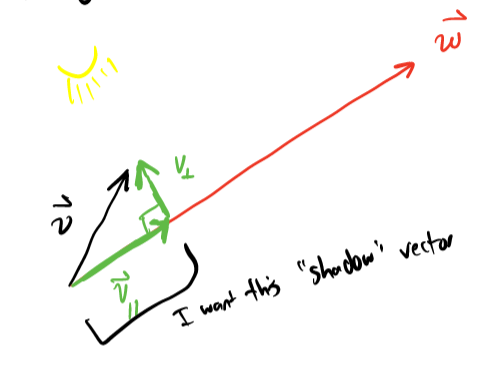
\includegraphics[width = 0.75\textwidth]{orthoproject.png}
\end{center}
Given the above figure, we are trying to find the
vector that is parallel (goes in the same direction
as vector $ \vec{w}$ ).
\begin{itemize}
  \item Notice how, much like in anything that is
        related to \textbf{multivariable calculus}, that
        we can generally form a \textbf{triangle}.
  \item In this case, we are able to create
        a triangle based on our original vector $ \vec{v}$
        that has a component that is perpendicular to
        $ \vec{w}$ but also parallel to $ \vec{w}$.
        This parallel vector will the basis of this
        concept of \textbf{orthogonal projection.}
\end{itemize}

Let us declare some variables first:
\[ \textrm{let $ \overrightarrow{v_{||}}$ be a leg of $ \vec{v}$
    that is parallel to $ \vec{w} $}\]
\[ \textrm{let $ \overrightarrow{v_{\perp}}$ be a leg of
    $ \vec{v}$ that is perpendicular or
  \textbf{orthogonal} to $ \vec{w}$}\]

Given these two variables as well as their relationships
between $ \vec{v}$ and $ \vec{w}$, we can make
some assertions.
\begin{enumerate}
  \item First, we know that $ \vec{v_{||}}$, since
        it is parallel to $ \vec{w}$ must be a
        \textbf{scaled down version of $ \vec{w}$}.
        This would make it a \textbf{scalar multiple
        of $ \vec{w}$}. Therefore, if we let $ a $ be
        some scalar, we know that
        \[ \overrightarrow{v_{||}} = a \cdot \vec{w}\]
  \item Second, we know that $ \vec{v_{\perp}}$
        is \textbf{orthogonal} to vector $\vec{w}$,
        therefore we know that the dot product
        between $ \vec{v_{\perp}}$ and $ \vec{w}$ must
        be equal to 0, since according to the definition
        of a dot product, two vectors are orthogonal
        if and only if their dot product is equal to 0.
        \[ \overrightarrow{v_{\perp}} \cdot \vec{w} = 0 \]
\end{enumerate}
Using all of this information, we are able to answer
the question, what is the value of $ a$? How can we
evaluate for the leg of the vector $ \vec{v}$ that is
parallel to vector $ \vec{w}$?

\subsection{Orthogonal Projection Proof}
\[ \vec{v} \cdot \vec{w} = \overrightarrow{v_{||}} \cdot
  \vec{w} + \overrightarrow{v_{\perp}} \cdot{w}\]
Since we know that $ \overrightarrow{v_{\perp}}
\cdot \vec{w} $ are perpendicular to each other, then
we know that they equal 0.
\[ \Rightarrow \vec{v} \cdot \vec{w} = \overrightarrow{v_{||}} \cdot
  \vec{w}  \]
Now, we are able to replace $ \overrightarrow{v_{||}}$
with the fact that we know that  $ \overrightarrow{v_{||}} =
a \cdot \vec{w}$ or that the parallel component of
vector $ \vec{v}$ is just a scaled version of
vector $ \vec{w}$.
\[ \Rightarrow \vec{v} \cdot \vec{w} =
(a \cdot \vec{w}) \cdot \vec{w}\]
By applying vector properties, we know that we can just
\textbf{move the parentheses} around.

\[ \Rightarrow \vec{v} \cdot \vec{w} =
  a \cdot (\vec{w} \cdot \vec{w})\]
\[ \Rightarrow a = \frac{\vec{v} \cdot \vec{w}}
  {\vec{w} \cdot \vec{w}}\]
\[ \Rightarrow \overrightarrow{v_{||}} = a
  \cdot w \]
\[ \Rightarrow \overrightarrow{v_{||}} =
\Biggr( \frac{\vec{v} \cdot \vec{w}}
{\vec{w} \cdot \vec{w}} \Biggr) \cdot
\vec{w} \]
From this, we know that $ \vec{v_{||}}$, which we
also know as \textbf{projection of vector $ v$ onto
  vector $ w $} is given by the following formula:
\[ proj_{w}v = \overrightarrow{v_{||}} =
  \Biggr(\frac{v \cdot w}{w \cdot w}\Biggr) \cdot \vec{w} \]
\subsection{Vector Projection}
\begin{center}
  \fbox{
    \parbox{\textwidth}{
      \begin{definition}
        Vector Projection (or the Vector Component)
      \end{definition}
      When given two
      vectors $ \vec{u} $ and $ \vec{v} $,
      the vector projection of $ u $ onto $ v$
      is the vector produced when  one vector $ u $ is
      resolved into two component vectors, one that
      is parallel to the second vector $ v $  and
      one that is perpendicular to the second
      vector $  v $. The vector that is parallel
      to the ``target'' vector is the \textbf{vector
        projection}.


    }
  }
\end{center}
\subsection{Vector Projection Intuition}
Based on the formula, recall how the vector
projection can be separated into two different
terms: the a scalar and the normalization of the vector being projected onto $ v $.
\[ proj_{v}u = \Biggr(\frac{u \cdot v}{||\vec{v}||^{2}} \Biggr)\vec{v} \]
\[ \Rightarrow proj_{v}u = \Biggr( \frac{\vec{u} \cdot \vec{v}}{||\vec{v}||}\Biggr) \cdot \Biggr( \frac{\vec{v}}{||\vec{v}||} \Biggr)\]
\[ \Rightarrow proj_{v}u = (\textrm{some scalar}) \cdot (\textrm{the unit vector or the \textbf{direction} of $\vec{v}$})\]

The idea here is that we are creating a vector
that is parallel (or technically overlapping) the
vector being projected on. Although the vector
is not necessarily the same magnitude of the
vector we are projecting, we can safely say
that the second term will always be the
\textbf{direction/unit vector of the vector
  being project onto}.

\subsection{The Angle Between Two Vectors}
\begin{center}
  \fbox{
    \parbox{\textwidth}{
      \begin{thm}
        The Angle Between Two Vectors (Theorem 1)
      \end{thm}
      The angle $ \theta $ between two nonzero
      vectors $ u = \langle u_{1}, u_{2}, u_{3} \rangle $
      and $ v = \langle v_{1}, v_{2}, v_{3} \rangle $
      is given by
      \[ \theta = \cos^{-1}\Biggr(\frac{u \cdot v}{||\vec{u}|||\vec{v}|||}\Biggr)\]
      \[ \Rightarrow \cos^{-1}\Biggr(\frac{u_{1}v_{1} +
        u_{2}v_{2} + u_{3}v_{3} }{||\vec{u}|||\vec{v}|||}\Biggr)\]
    }
  }
\end{center}
\subsection{The Proof of the Angle Between Two
  Vectors}
TODO





\section{Dot Product Properties and Vector Properties}
\begin{center}
  \fbox{
    \parbox{\textwidth}{
      \textbf{Properties of Dot Product and
        Vectors.} \\
      Let $ u = \langle u_{1}, u_{2}, u_{3} \rangle $,
      $ v = \langle v_{1}, v_{2}, v_{3}
      \rangle $, and $ c $ be a scalar

        \begin{enumerate}
          \item $ u \cdot v = v \cdot u $
          \item $ ku \cdot v = u \cdot kv = k(u \cdot v)$
          \item $ u \cdot (v + w) = u \cdot u \cdot w $
          \item $u \cdot u = ||\vec{u}||^2$
          \item $ 0 \cdot u = 0 $

        \end{enumerate}


    }
  }
\end{center}
\section{Proofs of the Properties of Dot Products}
TODO





\subsection{Scalar Component and the Scalar Projection}
\begin{center}
  \fbox{
    \parbox{\textwidth}{
      \begin{definition}
        Scalar Components/ Scalar Projection
      \end{definition}
      \textbf{Notation.}
      \[ comp_{v}u, \textrm{ or the ''scalar
          component of u onto  v`` }\]
      \textbf{Formula.}
      \[ comp_{v}u = \frac{u \cdot v}{||v||}\]
      \textbf{Explanation.} \\
      \[ \textrm{Let $comp_{v}u$ be the \textbf{scalar
          component of u onto v} }\]
      The magnitude of a vector that is projected
      onto another vector. If we divide the projection
      fromula into two terms: the magnitude of the
      resulting vector and the direction of the resulting
      vector (which is parallel to the vector being
      projected onto), we get the following formula:
      \[ proj_{v}u = (\textrm{magnitude of resulting
        vector}) \times (\textrm{direction of $\vec{v}$})\]
      \[ \Rightarrow proj_{v}u = \Biggr( \frac{u \cdot v}{||\vec{v}||} \Biggr) \cdot
        \Biggr( \frac{v}{||v||} \Biggr)\]

      \[ comp_{v}u = \Biggr( \frac{u \cdot v}{||v|| } \Biggr)\]
    }
  }
\end{center}
\subsection{Scalar Component Intuition}
TODO

\section{Summary}
In this chapter, we learned about the idea of the
\textbf{Dot Product}, as well as both of its
algebraic and geometric representations. Most importantly,
however, we leanred how to apply the dot product to
various different sitautions.
\begin{enumerate}
  \item
\end{enumerate}





\subsection{Important Formulas}
\begin{center}
  \fbox{
    \parbox{\textwidth}{
      \textbf{Formulas Involving Dot Product}
      \begin{enumerate}
        \item Algebraic Formulation of Dot Product
              \[ \vec{u} \cdot \vec{v} = u_{1}v_{1} +
              u_{2}v_{2} + u_{3}v_{3}\]
        \item Geometric Formulation of Dot Product
              \[ \vec{u} \cdot \vec{v} =
              ||\vec{u}|| \cdot ||\vec{v}|| \cdot \cos{\theta} \]
        \item Dot Product to Angle Formula
              \[ \cos{\theta} = \frac{u \cdot v}
              {||\vec{u}|| \cdot ||\vec{v}||}\]
        \item Vector Projection Formula
              \[ proj_{v}u = \frac{u \cdot v}{v} \cdot \frac{v}{||\vec{v}||}\]
        \item Scalar Projection (or Scalar Component) Formula
              \[ comp_{v}u = \frac{u \cdot v }{||\vec{v}||}\]

      \end{enumerate}
    }
  }
\end{center}

% Chapter 12.4: The Cross Product
\chapter{12.4: The Cross Product}
\section{Reminders}
TODO
\section{Objectives}
\begin{enumerate}
  \item Compute the cross product of two given
        vectors using \textbf{determinants}
  \item Geometrically interpret the
        magnitude and direction of the cross product
        of two given vectors
  \item Perform elementary vector operations
        \begin{itemize}
          \item Vector Addition
          \item Scalar Multiplication
          \item Dot Product
                \item Cross Product
        \end{itemize}

\end{enumerate}

\section{Recall}
Recall that in the last lecture, we discussed the
\textbf{dot product}, which had both an \textbf{algebraic}
definition as well as a \textbf{geometric} definition
\begin{itemize}
  \item Whenever we were finding the algebraic
        dot product, we were just multiplying the components
        and finding their sum
        \[ \vec{v} \cdot \vec{u} ~ = ~
        v_{1}u_{1} + v_{2}u_{2} + v_{3}+u_{3} \]

        We learned that this scalar actually represented
        a lot more than it let on. In fact, the
        \textbf{scalar that results from a dot product}
        actually represents the product of both vectors'
        magnitudes as well as the cosine of the angle
        between them:
        \[ \vec{v} \cdot \vec{u} ~ = ~
        || \vec{v} || \cdot || \vec{u} || \cdot
        \cos{\theta} \]

        where, of course, $ \theta $ represents the angle
        between the vectors $ v $ and $ u $.
        \\
        \par We also see the angle between two vectors
        $ \theta $ represented by the following formula

        \[ \cos{\theta} =
        \frac{\vec{v} \cdot \vec{u}}{||\vec{v}|| ||\vec{u}||}
        \]

  \item We also learned about \textbf{projection},
        which is the idea of taking a vector $ v $ and
        then imposing it onto another vector $ u $.
        Imagine that we were just ``flattening'' a vector
        onto another, preserving its length/magnitude
        while maintaining another vector's direction.
        \[ proj_{v}u =
        \frac{\vec{v} \cdot \vec{u}}{\vec{v} \cdot \vec{v}} \vec{v} \]
        which can also be represented as
        \[ \Rightarrow \Biggr(
        \frac{\vec{u} \cdot \vec{v}}{||\vec{v}||}
        \Biggr)
        \cdot
        \Biggr(
        \frac{1}{||\vec{v}||}
        \Biggr) \vec{v}
        \]
        where the first term $ \frac{\vec{v} \cdot \vec{u}}{||\vec{v}||}$ represents the
        \textbf{scalar component of v} and the second
        term $ \Biggr( \frac{1}{||\vec{v}||}\Biggr) \vec{v} $
        represents the \textbf{unit vector of $ \vec{v} $}.


\end{itemize}

\section{Motivation}
In the former lectures, we have learned about
\textbf{vectors} as well as numerous operations
to perform ont hem

\begin{itemize}
  \item Vector Addition/Subtraction $ \rightarrow $ vectors
  \item Scalar Multiplication $ \rightarrow $ vector
  \item Dot Product $ \rightarrow $ scalar
\end{itemize}

What if there was such an operation that we were able
to \textbf{multiply} two vectors together?

\section{Cross Product}
\begin{center}
  \fbox{
    \parbox{\textwidth}{
      \begin{definition}
        Cross Product
      \end{definition}
      The cross product of two vecturs $ \vec{v} $
      and $ \vec{u} $, $ (\vec{v} \times \vec{u}) $, is
      the geometrically defined by the following vector:
      \[ \vec{v} \times \vec{u} := ||\vec{v}||||\vec{u}||
        \cdot \sin{\theta} \cdot \vec{n} \ \]
      where vector $ \vec{n} $ is the \textbf{normal unit
        vector} perpendicular to the plane spanned by
      $ \vec{v} $ and $ \vec{u} $, which is chosen
      accordingly by the right hand rule.
      \\ \\
      \textbf{Book Definition.}
      The cross product $ u \times v $ or ``u
      cross v'' is the vector
      \[ u \times v = (|u||v|\sin{\theta})n \]

      \textbf{Layman Definition.}
      \\
      The cross product is the reuslting vector
      $ \vec{n} $, which is a vector that is orthogonal
      toe the plane of which $ \vec{v} $ and $ \vec{u} $
      occupy, and of which whose magnitude is determined
      by the product of the magnitude of $ \vec{v} $ and
      $ \vec{u} $, and the value of the angle betwen
      the two vectors that span the plane.
    }
  }
\end{center}

\begin{center}
  \fbox{
    \parbox{\textwidth} {
      \begin{definition}
        Parallel Vectors
      \end{definition}
      Nonzero vectors $ u $ and $ v $ are parallel
      \textbf{if and only if} $ u \times v = 0 $
    }
  }
\end{center}
\textbf{TODO: Insert Picture from Tablet}
\subsection{Observations of the Cross Product}
TODO

\section{Properties of the Cross Product}
\begin{center}
  \fbox{
    \parbox{\textwidth} {
      \begin{definition}
        Propeties of the Cross Product
      \end{definition}

      If $u $, $v$, and $w$ are any vectors and $r$,
      $s$ are any scalars, then

      \begin{enumerate}
        \item $ ru \times sv = rs(u \times v)$
        \item $u \times (v + w ) = u \times v + u \times w $
        \item $v \times u = -(u \times v)$
        \item $(v + w) \times u = v \times u + w \times u$
        \item $0 \times u = 0$
        \item $u \times (v \times w) =
              (u \cdot w)v - (u \cdot v)w$
      \end{enumerate}

    }
  }
\end{center}

\section{Parallelograms and the Magnitude of a Cross Product}
\begin{center}
  \fbox{
    \parbox{\textwidth} {
      \begin{definition}
        Area of a Parallelogram bounded by $ u $ and $ v $
      \end{definition}
      Given that $ n $ is a unit vector, we can
      think of the magnitude of $ u \times v $ as
      \[ | u \times v | = |u||v||\sin{\theta}||n| =
      |u||v|\sin{\theta}\]
    }
  }
\end{center}

\section{Algebraically Evaluating the Cross Product}
\begin{center}
  \fbox{
    \parbox{\textwidth} {
      \begin{definition}
        Calculating the cross Product as a Determinant
      \end{definition}
      If $ u = u_{1}i + u_{2}j + u_{3}k $ and
      $ v = v_{1}i + v_{2}j + v_{3}k $, then
      \[ u \times v =
        \begin{vmatrix}
          i & j & k \\
          u_{1} & u_{2} & u_{3} \\
          v_{1} & v_{2} & v_{3}
        \end{vmatrix}\]
      \[ \Rightarrow u \times v =
      \begin{pmatrix}
        u_{2} & u_{3} \\
        v_{2} & v_{3}
      \end{pmatrix}i -
    \begin{pmatrix}
      u_{1} & v_{3} \\
      v_{1} & v_{3}
    \end{pmatrix}j +
    \begin{pmatrix}
      u_{1} & u_{2} \\
      v_{1} & v_{2}
    \end{pmatrix}k
\]
    }
  }
\end{center}

% Chapter 12.5 Lines in Space
\chapter{12.5: Lines in Space (04/07/23 - 04/10/23)}
\section{Reminders}
\begin{itemize}
        \item
\end{itemize}

\section{Objectives}
In this section, we want to be able to do the
following:
\begin{itemize}
  \item Be able to write equations for lines
        and line segments in $ \R^{3} $ space
        using scalar and vector products
\end{itemize}

\section{Motivation}
Recall in the last lessons we have been
learninge exclusively about vectors as well
as how we are able to manipulate them in order
to get different objects in space.
\begin{itemize}
  \item For example, we have learned that the
        \textbf{Dot Product} is a function that takes
        in two vectors $ \vec{v}$ and $ \vec{u}$
        and returns some scalar.
        \[ \vec{v} \cdot \vec{u}  \]
        Much like anything in multivariable calculus,
        we actually have to consider that a lot of the
        concepts we learn are \textbf{multi-dimensional}.
        In this case, we must understand that the
        \textbf{dot product} has both a \textbf{algebraic}
        and \textbf{geometric} definition.
        \par Algebraically, we can think of the dot product
        as the following equation:
        \[ \textrm{let $ \vec{v} = \langle v_{1}, v_{2}, v_{3} \rangle $}\]
        \[ \textrm{let $ \vec{u} = \langle u_{1}, u_{2}, u_{3} \rangle$}\]
        \[ \Rightarrow
        \vec{v} \cdot \vec{u} ~ = ~ v_{1}u_{1} + v_{2}u_{2}
        + v_{3}u_{3} \]
        \par Geometrically, we can think of the
        \textbf{dot product} as the \textbf{angle between
        two vectors, but scaled based on the magnitude
        of the vectors.}
        \[ \textrm{let $ \vec{v} = \langle v_{1}, v_{2}, v_{3} \rangle $}\]
        \[ \textrm{let $ \vec{u} = \langle u_{1}, u_{2}, u_{3} \rangle$}\]
        \[ \Rightarrow \vec{v} \cdot \vec{u} ~ = ~
        ||\vec{v}|| \cdot ||\vec{u}|| \cdot \cos{\theta}\]
        \par Of course, there are a few implications and
        use cases of the dot product both algebraically
        and geometrically
        \begin{itemize}
          \item If $ \vec{v} \cdot \vec{u} = 0 $,
                then we know that the vectors $ v $ and
                $ u $ are \textbf{orthogonal or
                perpendicular}, which makes sense,
                since if we were to find some value
                $ \cos{\theta} = 0$, then we would have
                $ \theta = \frac{\pi}{2} $, which is of
                course, a right angle.
                \item
        \end{itemize}

        \textbf{TODO: Include Graphics that Visualizes
        this relationship}

\end{itemize}

\subsection{Lines in $ \R^{2}$}
\fbox{
  \parbox{\textwidth} {
    \begin{definition}
      Lines in $ \R^{2} $
    \end{definition}
    \textbf{Layman's Definition.} \
  }
}
\subsection{Intuition Behind Lines in $ \R^{2} $}

\subsection{Lines in $ \R^{3 }$}
\begin{center}
\fbox{
  \parbox{\textwidth} {
    \begin{definition}
      Lines in $ \R^{3} $
    \end{definition}
    A \textbf{vector equation for the line} $ L$
    through the point $ P_{0} $ where $ P_{0}(x_{0},
    y_{0}, z_{0})$ and parallel to $ v $ is
    given by
    \[ \vec{r}(t) = r_{0} + t \cdot \vec{v} ~ \textrm{
          where }-\infty <
    t < \infty \]
    where $ r $ represents the position vector
    of a point $ P(x, y, z)$ on the line $ L$ from
    the point $ P_{0}$ and $r_{0}$ is the
    position vector of $ P_{0}(x_{0}, y_{0}, z_{0})$.
    We also let $ \vec{v} $ be some vector that is
    \textbf{parallel} to our desired direction.
    \textbf{Layman's Definition.} \
  }
}
\end{center}
\subsection{Intuition Behind $ \R^{3} $ Lines}
TODO

\section{Parametric Equations of a Line}
Given any vector equation of a line, we notice
that everything can be put into terms of each
of the individual directions $ x, y, z$.
\begin{center}
  \fbox{
    \parbox{\textwidth} {
      \begin{definition}
        Parametric Equations of a Line
      \end{definition}
      The \textbf{standard parameterization of the line}
      through $ P_{0}(x_{0}, y_{0}, z_{0})$ parallel
      to $ v = v_{1}i + v_{2} j + v_{3}k $ is
      \[ x = x_{0} + t \cdot v_{1}~ \textrm{   where }
      ~ -\infty < t < \infty \]
      \[ y = y_{0} + t \cdot v_{2}~ \textrm{   where }
      ~ -\infty < t < \infty \]
      \[ z = z_{0} + t \cdot v_{3}~ \textrm{   where }
      ~ -\infty < t < \infty \]
      \textbf{Layman's Definition.} \
    }
  }
\end{center}
\section{Solving Lines in Space Problems}
\subsection{Distance from a Point to a Line in Space}
\begin{center}
  \fbox{
    \parbox{\textwidth} {
      \begin{definition}
        Distance from a Point $ S $ to a Line
        Through $ P $ Parallel to $ v $
      \end{definition}

      \[ d = \frac{|\overrightarrow{PS} \times \vec{v} |}{|\vec{v}|}\]

    }
  }
\end{center}




\subsection{2-D Lines versus 3-D Lines}
Whenever we were defining lines in $ \R^{2}$, we
were always thinking of these lines as an
a set of points with two defining characteristics:
\begin{itemize}
  \item Some point $ P_{0} $ that the line
        intersected
  \item Some slope or direction $ m $ that the
        line went in
\end{itemize}

With the intuition that lines in two-dimensional space
were defined by the points they intersectd as well
as their \textbf{slope}, which we can think of as
the \textbf{change in x and the change in y over time},
we can apply the same general principals to vectors in
three-dimensional space.
\subsection{3-D Lines}
Three dimensional lines, by comparison, are also
defined by some point that the line goes through
as well as a direction in which the line continues
infinitely. Instead of having a slope, however,
we like to think of the ``slope'' of a three-dimensional
line as a ``parallel'' vector, that doesn't necessarily
represent the actual line, but the \textbf{behavior}
of our current line.
\par A three-dimensional line is defined by the following
terms:
\begin{itemize}
  \item An \underline{\textbf{initial point}} $ P_{0} $ or
        just $ P $.
  \item A \underline{\textbf{vector}} that defines
        the line's \textbf{direction} and \textbf{behavior},
        $ \overrightarrow{P_{0}P} $ or $ \overrightarrow{PQ}$, where $ P_{0} $ and
        represents the initial point and $ P $ and $ Q $
        represent \textbf{any point on the line}.

\end{itemize}
\subsection{3-D Line Summary}
Essentially, much like hte \textbf{two-dimensional line},
a \textbf{three-dimensional line} is defined by some
point $ P $ that the line goes through, as well as
a \textbf{directional vector} that starts from that
initial point $ P $ and extends to any point $ Q $ on
the line $ \overrightarrow{PQ} $.


% 12.5: Planes in Space
\chapter{12.5: Planes in Space (04/07/23 - 04/10/23)}
\section{Reminders}
\subsection{MATH\_226 Reminders (as of Saturday, April 22, 2023)}
\begin{enumerate}
  \item \textbf{Written Homework 4: Power Series} is
        due on \textbf{Monday, April 24, 2023.}
\end{enumerate}

\subsection{MATH\_230 Reminders (as of Saturday, April 22,
  2023)}
\begin{enumerate}
  \item
\end{enumerate}

\section{Objectives}
\begin{enumerate}
  \item Determine vector and component equations
  \item Produce non-zero vectors normal to a given plane
  \item Compute the distance from a point to a plane
        in space
  \item Determine whether two given planes coincide, intersect in a line, or are parallel

\end{enumerate}

\section{Motivation}
In the last seciton, we learned about \textbf{lines in space}, how
they're portrayed in two dimensions, as well as how they're portrayed in three dimensions.
We analyzed the relationship between lines in space as ewll as

\section{Planes in $ R^{3}$}
\subsection{Vector Equation of a Plane}
\fbox{
  \parbox{\textwidth} {
    \begin{definition}
      Vector Equation of a Plane
    \end{definition}
    The plane through $ P_{0}(x_{0}, y_{0}, z_{0})$
    that is normal to $ n = Ai + Bj + Ck $ is given
    by the equation
    \[ n \cdot \overrightarrow{P_{0}P} = 0 \]
    \textbf{Layman's Definition.} \
  }
}

\subsection{Component Equation of a Plane}
\begin{center}
  \fbox{
    \parbox{\textwidth} {
      \begin{definition}
        Component Equation of a Plane
      \end{definition}
          The plane through $ P_{0}(x_{0}, y_{0}, z_{0})$
    that is normal to $ n = Ai + Bj + Ck $ is given
    by the equation
    \[ A(x-x_{0}) + B(y -y_{0}) + C(z - z_{0}) = 0 \]
      \textbf{Layman's Definition.} \
    }
  }
\end{center}

\subsection{Simplified Component Equation of a Plane}
\begin{center}
  \fbox{
    \parbox{\textwidth} {
      \begin{definition}
        Simplified Component Equation of a Plane
      \end{definition}
      The plane through $ P_{0}(x_{0}, y_{0}, z_{0})$
    that is normal to $ n = Ai + Bj + Ck $ is given
    by the equation
    \[ Ax + By + Cz = D\]
      \textbf{Layman's Definition.} \
    }
  }
\end{center}
\subsection{Intuition Behind Planes}
TODO
\section{Types of Problems and How to Solve Them}
\subsection{Determining the Intersection Between
  Two Planes}
\begin{center}
  \fbox{
    \parbox{\textwidth} {
      \textbf{Algorithm.} \textit{Line of Intersection Between Two Planes} \\ \\
      Given two planes $ P_{1} $ and $ P_{2}$
      \begin{enumerate}
        \item Determine what the normal vectors of $ P_{1}$ and
              $P_{2}$ are
        \item Find the vector parallel to the vector that
              is orthogonal to the normal vectors of $ P_{1}$
              and $ P_{2}$
        \item Evaluate a point that exists on the line
              by literally plugging in any value into
              the system of equatiosn formed by the
              two different planes.
              \begin{enumerate}
                \item The idea here is that, since
                      a line expands infinitely in
                      both directions, that
                      we must be able to find
                      some point in which the x
                      coordinate is 4, for example.
                      There is no rhyme or reason
                      to anything here, literally just
                      plug in some numbers
                      and you will most likely be
                      fine.
              \end{enumerate}


        \item Write equation using the direction vector
              (which is the vector that is parallel to the
              vector normal to the normal vectors of $ P_{1}$ and
              $P_{2}$).
      \end{enumerate}

    }
  }

\end{center}
\subsection{Line of Intersection Between Two Planes Intuition.}
Whenever we are determining the line of intersection
between two planes, it is important to remember how this
geometrically works in relation to what we know about
planes.
\begin{enumerate}
  \item Recall that planes are represented by two
        different components
        \begin{enumerate}
          \item Some point that exists on the plane
          \item Some vector $ \vec{n}$ that
                is parallel to the vector that is
                normal to the plane
        \end{enumerate}
  \item Using this knowledge, we are able to make
        some implications
        \begin{enumerate}
          \item First, it is important for us to
                remember that whenever two planes
                are parallel, then their normal
                vectors must also be parallel to each
                other
          \item Likewise, if two planes
                were to intersect, that must mean
                that their normal vectors \textbf{must
                also be intersecting}. We
                can use this information to
                actually find the direction in
                which the two vectors intersect
                (imagine that the two vectors
                are intersecting in two-dimensional
                space and that we are trying to
                find the vector that goes ``through''
                that point of intersection).
          \item Of course, in order to find
                this point of intersection, we
                think of the cross product,
                since through the cross product,
                we are able to find a vector that is
                normal to the plane spanned
                by the two constituent vectors,
                which, in this case,
                are the two vectors that are normal
                to the planes.
          \item This normal vector will
                serve as the direction vector
                for our line of intersection.

        \end{enumerate}


\end{enumerate}

\subsection{Finding the Equation of a Plane Given
  Three Points}
\begin{center}
      \dfn{Algorithm: Finding the Equation of a Plane Given Three Points}
      {\begin{enumerate}
        \item Create two vectors from the three given points $ \overrightarrow{PQ}$ and $ \overrightarrow{PO}$

      \item Find the cross product between the two
      newly created vectors $ \overrightarrow{PQ}$ and
      $ \overrightarrow{PO}$
      \[ \overrightarrow{PQ} \times \overrightarrow{PO} \]
      \item Let the result of the cross product
      be the vector parallel to the normal vector
      spanned by the plane $ \vec{n} $
      \item Create the equation using any given point
      plus the vector parallel to the normal vector $
      \vec{n}$
      \end{enumerate}
       }
\end{center}
\subsection{Intuition for Finding the Equation of a Plane
Given Three Points.}
        When finding the equation of a plane
        given three points, its important to consider
        what exactly we need to define a plane.
        \begin{enumerate}
          \item First, we need a vector that
                is parallel to the vector that
                is normal to the plane $ \vec{n}$
          \item Second, we just need a point
                that exists on the plane
        \end{enumerate}
        When we are given three points we are able to
        meet all of these different requirements.
        \begin{enumerate}
          \item With three points, we are able to
                create two vectors that could exist
                on the plane, and then we are able
                to find their \textbf{cross product} and
                let this result be the vector that
                is parallel to the vector that is
                normal to the plane $ \vec{n}$.
          \item The only thing that remians is just
                using a point on the plane, and
                we are literally given three points of
                potential comparison.
        \end{enumerate}


\subsection{Determining the Distance from a Point to a Plane}
\begin{center}
        \dfn{Algorithm:
        Distance from a Point to a Plane}
      {\begin{enumerate}
        \item Determine a position vector between the
              point in space and a point on the plane.
        \item Using the position vector from the
              point in space and the point on the plane,
              find the \textbf{projection of the position
              vector onto the vector that is parallel
              to the normal vector of the plane } $ \vec{n}$.
      \end{enumerate}
      \[ \textrm{let $ P$ be a point in space}\]
      \[ \textrm{let a plane $ M $ be defined as }\]
      \[ M = \vec{Q} + \vec{n} t \]
      \[ \overrightarrow{PQ} = \langle Q_{1} - P_{1}, Q_{2} - P_{2}, Q_{3} - P_{3} \rangle\]
      \[ proj_{n}\overrightarrow{PQ} = \frac{\overrightarrow{PQ} \cdot \vec{n} }{||\vec{n}|| ||\vec{n}||} \vec{n}   \]
      \textbf{Layman's Definition.} \\
      The idea here is that, much like
      other distanc eproblems, we
      want to find any distance from the
      point to the plane, then we just want to
      \textbf{put it into terms of the normal vector}.
    }
\end{center}


\subsection{Intuition Behind Determining the Distance from a Point to a Plane}
When we are given a distance question between anything--
whether it be a point to a line, a line to a plane,
or a plane to a plane, it is important to \textbf{always}
consider the idea of \textbf{projectoin.} Projection
will always be the basis of finding the distance,
since, at the end of the day, we want to be able to
take \textit{any distance we find between the objects},
and project it onto the least possible distance--
\textbf{the normal vector.}




\chapter{(TODO) 11.6: Conic Sections (04/12/23)}
\section{Reminders (as of 04/23/23)}
\subsection{MATH\_230-1 Reminders}
\begin{itemize}
  \item \textbf{MyLab Math 9: Curves in Space and Their
        Tangents} is due \textbf{tonight, April 23, 2023}.
  \item \textbf{Midterm 1} is on \textbf{Tuesday, April
        25, 2023}.

\end{itemize}
\subsection{MATH\_226-0 Reminders}
\begin{itemize}
  \item \textbf{MyLab Math 11: Manipulation of Series}
        is due on \textbf{Tuesday, April 25, 2023}.
  \item \textbf{Written Homework 4: Power Series} is due
        \textbf{tomorrow, Monday April 24, 2023}
\end{itemize}




\section{Objectives}
\begin{enumerate}
  \item Be able to algebraically and geometrically
        understand the three conic sections
  \item Be able to graph all three conic sections

\end{enumerate}

\section{Motivation}
In order to
\section{Circles}
\begin{center}
  \fbox{
    \parbox{\textwidth} {
      \begin{definition}
        Circles
      \end{definition}
      \[ x^{2} + y^{2} = 1 \]
      \[ (x-h)^{2} + (y-k)^{2} = r^{2}\]
    }
  }
\end{center}

\section{Ellipses}
\begin{center}
  \fbox{
    \parbox{\textwidth} {
      \begin{definition}
        Ellipses
      \end{definition}
      \[ \frac{(x-h)^{2}}{a^{2}} + \frac{(y-k)^{2}}{b^{2}} = 1\]
    }
  }
\end{center}
\section{Parabolas}
\begin{center}
  \fbox{
    \parbox{\textwidth} {
      \begin{definition}
        Parabolas
      \end{definition}
      \[ y = x^{2}\]
      \[ x = y^{2}\]

    }
  }
\end{center}
\section{Hyperbolas}
\begin{center}
  \fbox{
    \parbox{\textwidth} {
      \begin{definition}
        Hyperbolas
      \end{definition}
      \[ \frac{(x-h)^{2}}{a^{2}} - \frac{(y-k)^{2}}{b^{2}} = 1 \]
      \[ \frac{(y-k)^{2}}{a^{2}} - \frac{(x-h)^{2}}{b^{2}} = 1 \]
    }
  }
\end{center}


% Chapter 12.6: Cylinders and Quadric Surfaces
\chapter{(TODO) 12.6: Cylinders and Quadric Surfaces (04/14/23)}
\section{Reminders (as of 04/23/23)}
\subsection{MATH\_230-1 Reminders}
\begin{itemize}
  \item \textbf{MyLab Math 9: Curves in Space and Their
        Tangents} is due \textbf{tonight, April 23, 2023}.
  \item \textbf{Midterm 1} is on \textbf{Tuesday, April
        25, 2023}.

\end{itemize}
\subsection{MATH\_226-0 Reminders}
\begin{itemize}
  \item \textbf{MyLab Math 11: Manipulation of Series}
        is due on \textbf{Tuesday, April 25, 2023}.
  \item \textbf{Written Homework 4: Power Series} is due
        \textbf{tomorrow, Monday April 24, 2023}
\end{itemize}

\section{Objectives}
\begin{enumerate}
  \item Sketch the graph of various cylinders
  \item Graph the \textbf{six} quadric surfaces by hand
  \item Understand the usefulness of the coordinate plane
        traces as well as how to find them

\end{enumerate}

\section{Motivation}

\section{The Six Types of Quadric Surfaces and Cylinders}
\subsection{Ellipsoid}
\fbox{
  \parbox{\textwidth} {
    \begin{definition}
      Ellipsoid
    \end{definition}
    TODO
  }
}
\subsection{Hyperboloid of One Sheet}
\fbox{
  \parbox{\textwidth} {
    \begin{definition}
      Hyperboloid of One Sheet
    \end{definition}
    TODO
  }
}
\subsection{Hyperboloid of Two Sheets}
\begin{center}
  \fbox{
    \parbox{\textwidth} {
      \begin{definition}
        Hyperboloid of Two Sheets
      \end{definition}
      TODO
    }
  }
\end{center}
\subsection{Elliptic Paraboloid}
\begin{center}
  \fbox{
    \parbox{\textwidth} {
      \begin{definition}
        Elliptic Paraboloid
      \end{definition}
      TODO
    }
  }
\end{center}
\subsection{Hyperbolic Paraboloid}
\begin{center}
  \fbox{
    \parbox{\textwidth} {
      \begin{definition}
        Hyperbolic Paraboloid
      \end{definition}
      TODO
    }
  }
\end{center}
\subsection{Elliptical Cone}
\begin{center}
  \fbox{
    \parbox{\textwidth} {
      \begin{definition}
        Elliptical Cone
      \end{definition}
      TODO

    }
  }
\end{center}

\chapter{(TODO) 11.3: Polar Coordinates (04/17/23)}
\section{Reminders (as of 04/23/23)}
\subsection{MATH\_230-1 Reminders}
\begin{itemize}
  \item \textbf{MyLab Math 9: Curves in Space and Their
        Tangents} is due \textbf{tonight, April 23, 2023}.
  \item \textbf{Midterm 1} is on \textbf{Tuesday, April
        25, 2023}.

\end{itemize}
\subsection{MATH\_226-0 Reminders}
\begin{itemize}
  \item \textbf{MyLab Math 11: Manipulation of Series}
        is due on \textbf{Tuesday, April 25, 2023}.
  \item \textbf{Written Homework 4: Power Series} is due
        \textbf{tomorrow, Monday April 24, 2023}
\end{itemize}



\section{Objectives}
\begin{enumerate}
  \item Be able to differentiate between poloar
        coordinates and Cartesian coordinates
  \item Be able to relate polar coordinates to
        Cartesian coordinates
  \item Graph polar coordinate functions

\end{enumerate}

\section{Motivation}
In the previous sections, we have
learned about different ways to depict
sets of coordinates in space
\begin{itemize}
  \item Vectors
  \item Lines
  \item Planes
\end{itemize}
However, we have done all of this using
the \textbf{Cartesian or Rectangular
  Coordinate System}, which is our
system that determines movements in
graphs through the $ x $, $ y$, and $ z$
dimensions. There are, of course,
other ways to explore this movement,
though, such as through the
\textbf{Polar System}, which,
instead of basing two-dimensional
movement as movement in the
$ x $ and $ y $, dimensions,
calculates movement as a function
of magnitude $ r $ and angle $ \theta $.
We will find that these concepts of
$ r $ and $ \theta $ can be
applied to normal rectangular
system equations and, in
investigating the relationships
between the Cartesian and Polar
Systems, we are able to
develop functions direclty
out of rectangular movement.


\section{Polar Coordinate Movement }
\begin{center}
  \fbox{
    \parbox{\textwidth} {
      \begin{definition}
        Polar Coordinate System
      \end{definition}
      Fix an origin $ O $ (which we call the pole)
      and an create an \textbf{initial ray} from
      the pole $ O $ (which will just be a
      ray across the positive x-axis).
      We are able to locate
      any point $ P $ in the coordinate
      system by assigning it to a polar
      coordinate pair $ (r, \theta)$ in
      which $ r $ gives the directed
      distance from $ O $ to $ P $,
      and $ \theta $ gives the directed
      angle from the initial ray
      to the ray $ \overrightarrow{OP}$.
      We label this point $ P $ as
      $ P(r, \theta)$.

    }
  }
\end{center}

\section{Switching Between Polar Coordinates
  and Cartesian Coordinates}
\begin{center}
  \fbox{
    \parbox{\textwidth} {
      \begin{definition}
        Common Cartesian/Polar Translations
      \end{definition}
      We are able to switch between
      polar and cartesian coordinates
      based on the following known
      transformations
      \[ x = r\cos{\theta}\]
      \[ y = r\sin{\theta}\]
      \[ r^{2} = x^{2} + y^{2}\]
    }
  }
\end{center}

\subsection{Common Strategies for Switching
  Between Polar Coordinates}
Whenever we are trying to convert
Cartesian equations into Polar Equations,
we will find that there are a number
of strategies to convert an equation
from one coordinate system to the next.
\par For example, what if you had
to convert
\[ r\sin{\theta} ~ \textrm{to Cartesian}\]
\[ r^{2}\sin^{2}{\theta} ~ \textrm{to Cartesian}\]
\[ y = x^{2} ~ \textrm{$\forall x \neq 0$ }\]

\subsection{Direct Substitution}
\begin{remark*}[(1)]
  Convert the following Polar Equation into a
  Cartesian Equatino
  \[ r\sin{\theta} = 3 \]
  When we approach this problem, it is important
  to \textbf{recall} the standard conversions
  we are given.\\
  \textbf{Recall.}
  \[ x = r\cos{\theta}\]
  \[ y = r\sin{\theta}\]
  \[ x^{2} + y^{2} = r^{2}\]
  From this, we can just \textbf{directly
    subsitute} some of these converisons.
  \[ r\sin{\theta} = 3\]
  \[ \Rightarrow y = 3 \]


\end{remark*}
\subsection{Multiplying $ r $ on Both Sides}
\begin{remark*}[2]
  Convert the following Polar Equation into
  a Cartesian Equation
  \[ \sin{\theta} = r\cos^{2}{\theta}\]
\end{remark*}
Unfortunately here, we don't have a particularly
easy way of substituting the knowledge we know.
After all, all we can really think of doing is
separating the term on the right into something
we know, but then that would leave us with a
very messy looking equation. THerefore, what we
are able to do (or what we should consider)
doing is \textbf{multiplying both sides by $r$}.
\[ \Rightarrow \sin{\theta} = r\cos^{2}{\theta}\]
\[ \Rightarrow r \cdot \sin{\theta} = r \cdot r\cos^{2}{\theta}\]
\[ \Rightarrow r\sin{\theta} = r^{2}\cos^{2}{theta}\]
From here, now we have a lot of
information in which we are able to just
\textbf{substitute what we know}.
\[ \Rightarrow r\sin{\theta} = (r\cos{\theta})^{2}\]
\[ \Rightarrow y = x^{2} \]

\subsection{Tricks in Summary}
Evidently, in order to succeed in converting
Polar and Cartesian Equations, we just
have to look out for the following
terms:
\begin{enumerate}
  \item  $r\cos{\theta} = x$
  \item $r\sin{\theta} = y$
  \item $ \tan{\theta} = \frac{y}{x}$
  \item $r^2 = x^{2} + y^{2} $

\end{enumerate}

\begin{remark*}[3 (harder)]
  \[ \tan^{2}{\theta} - 1 = \frac{6}{r}\tan{\theta}\sec{\theta}
    + \frac{4}{r}\sec{\theta} \]
\end{remark*}

In this problem, we have an even
worse initial state than the previous
problem, since we are confronted
with a new term, \textbf{secant}.
However, as with most problems in algebra
and calculus, the best way to solve
something you don't know is to
\textit{break it into something you do
  know}.
\par In this, case we are going to first
\textbf{substitue all of the secants with
  reciprocals of $ \cos{\theta}$}.
\[ \Rightarrow \tan^{2}{\theta} - 1 = \frac{6}{r}\tan{\theta}
  \frac{1}{\cos{\theta}} + \frac{4}{r} \frac{1}{\cos{\theta}
  }\]
Then, we are just able to rewrite
$ \tan^{2}{\theta}$ as a functino of
sine and cosine.
\[ \Rightarrow \frac{\sin^{2}}{\cos^{2}} - 1
  = \frac{6}{r}\tan{\theta}\frac{1}{\cos{\theta}}+\frac{4}{r\cos{\theta}}\]

\[ \Rightarrow r \Biggr( \frac{\sin^{2}{\theta}}{\cos^{2}{\theta}}
    -1 \Biggr) = \Biggr( \frac{6}{r}\tan{\theta}\frac{1}{\cos{\theta}}
    + \frac{4}{r\cos{\theta}}\Biggr) \cdot r
\]
\[ \Rightarrow
  r\sin^{2}{\theta} - r = 6\tan{\theta}\cos{\theta} + 4\cos{\theta}
\]
\[ \Rightarrow r\sin^{2}{\theta} - r
  = 6\sin{\theta} + 4\cos{\theta}\]
\[ \Rightarrow r^{2}\sin^{2}{\theta} - r^{2}
  = 6r\sin{\theta} + 4r\cos{\theta}\]
\[ \Rightarrow y^{2} - x^{2} - y^{2} = 6y + 4x \]

\[ \Rightarrow y^{2} - 6y -x^{2} - 4x = 0 \]
\[ \Rightarrow (y-3)^{2} -9 - (x+2)^{2} + 4 = 0 \]
\[ \Rightarrow (y-3)^{2} - (x+2)^{2} = 5 \]
% Chapter 13.1: Curves in Space and Their Tangents
\chapter{13.1: Curves in Space and their Tangents (04/19/23)}
\section{Reminders}
\subsection{MATH\_230-1}
\begin{enumerate}
  \item \textbf{MyLab Math 8: Polar Coordinates} is
        going to be due \textbf{tomorrow, Thursday, April
        19, 2023}.
  \item \textbf{Written Homework 2} is due
        \textbf{tonight, Wednesday, April 19, 2023}.
  \item \textbf{MyLab Math 9: Curves in Space
        and Their Tangents} is going to be due
        on \textbf{Sunday, April 23, 2023}.

\end{enumerate}
\subsection{MATH\_226-0}
\begin{enumerate}
  \item \textbf{MyLab 10: Radius and Interval of
        Convergence} is going to be due on
        \textbf{Friday, April 19, 2023}.
\end{enumerate}


\section{Objectives}
In this section, we want to be able to
understand how to portray curves as they
exist in space. Most importantly we want
to be able to understand the concept of
\textbf{parameterized equations} and
\textbf{vector-valued functions} and
how we are able to manipulate them and
understand them in space.
\begin{enumerate}
  \item Analyze a vector-valued function
        using limits, continuity, and the
        derivative
  \item Interpret the derivative of a
        vector-valued function
        \begin{itemize}
          \item Interpret the derivative of a
                vector-valued function
                in the context of particle
                motion
        \end{itemize}
  \item Analyze the velocity vectror
        of a particle to determine a particle's
        speed, direction, and accelration
  \item Fluently apply differentiation rules
        to vector-valued functions
  \item Show that the output of a
        vector-valued function of constant
        length is orthogonal to its
        derivative.

\end{enumerate}

\section{Recall}

\section{Motivation}

\section{Vector-Valued Functions and the
Parameterization of Plane Curves}

\begin{center}
  \fbox{
    \parbox{\textwidth} {
      \begin{definition}
        Vector-Valued Functions
      \end{definition}
      A function on a domain set $ D $ that
      assigns a \textbf{vector} for every
      element in $ D $.
      \[ r(t) = \overrightarrow{PQ} = f(t)\hat{i} +
        g(t)\hat{j} + h(t)\hat{k}\]
      \[ \Rightarrow \langle f(t), g(t), h(t) \rangle\]
      The functions $ f(t)$, $g(t)$, and $h(t)$ are known
      as \textbf{component functions}, notice that
      this is because they are \textbf{components}
      of the vector (recall that the \textbf{component
        form} of a vector is just the vector in terms of
      the standard unit vectors). \\
      For now, the domain of these functions will
      just be \textbf{real numbers}, while the
      actual graph of the function will represent a
      \textbf{curve in space}.
      \\ \\
      \textbf{Layman's Definition.} \\
      Essentially, a \textbf{vector-valued function}
      is just a function that takes in some
      number $ \in \R$ and outputs a \textbf{vector}.
      \par By contrast, \textbf{vector-valued functions}
      or \textbf{vector functions} are contrasted by
      \textbf{scalar functions}, which are functions
      on the domain set $ D \in \R $ that have a range
      $ \R \in \R $.
    }
  }
\end{center}


\begin{center}
  \fbox{
    \parbox{\textwidth} {
      \begin{definition}
        Parametric Equations
      \end{definition}
      If $ x $ and $ y $ are given as
      continuous functions
      \[ x = f(t); ~ y = g(t)\]
      over an interval $ I $ of $ t$-values,
      then the set of points
      \[ (x,y) = (f(t), g(t))\]
      defined by these equations is a
      \textbf{parametric curve}. From
      this, we know that the equations
      \[ x = f(t); ~ y = g(t)\]
      are \textbf{parametric equations}
      for this parametric curve.

      \par Given the closed interval
      $ I = [a, b]$
      the point A(f(a), g(a)) is known
      as the \textbf{initial point} of
      the parametric curve, while
      point B(f(b), g(b)) is known as the
      \textbf{terminal point} of the
      parametric curve.
    }
  }
\end{center}

\section{Methods for Sketching Parametric Curves}
\subsection{Method 1: Parametric Equation Tables}
TODO
\subsection{Method 2: Re-Writing Parametric Equations in
  Terms of $ x, y, z $}
TODO



\begin{center}
  \fbox{
    \parbox{\textwidth} {
      \begin{definition}
        Component Functions
      \end{definition}
      A \textbf{component function} is just
      a \textbf{component} of a vector $ \vec{v}$
      where, instead of being some constant,
      is a \textbf{function}.

      \[ \vec{v} = \langle f(t), g(t), h(t) \rangle\]

      This is in contrast to vector $ \vec{u}$, which
      has components that are constants.
      \[ \vec{u} = \langle 1, 2, 3  \rangle\]
      \textbf{Layman's Definition.} \\
      A component function is a component of a
      vector (representing the ``movement''of a
      vector), except, instead of being a constant
      number, is just a function.
    }
  }
\end{center}

\subsection{Examples of Vector-Valued Functions}
\begin{remark*}[1]
  Graph the vector-valued function
  \[ r(t) = \cos{t}\hat{i} + \sin{t}\hat{j} + t\hat{k}\]
\end{remark*}
Whenever we are looking at this function,
we first just need to \textbf{break everything down
  into its components}.
\par Remember, that this is a \textbf{vector-valued
  function}, so we can think of each
\textbf{component function} as being
representative of what the vector does
for a given $ t $. In this case,
we can contextualize the function like
so
\[ x = \cos{t}\]
\[ y = \sin{t}\]
\[ z = t \]
With some algebraic manipulation with the
component function of $ x $ and the
component function of $ y $, we can see that
our vector-valued function actually
satisfies the equation of a circle
if we ignore the behavior in the
z-axis.
\[ r(t) = \cos{t}\hat{i} + \sin{t}\hat{j} \]
\[ \Rightarrow x = \cos{t}; ~ y = \sin{t}\]
\[ x^{2} + y^{2} = \cos^{2}{t} + \sin^{2}{t} \]
\[ \Rightarrow \cos^{2}{t} + \sin^{2}{t} = 1 \]
We can see that a little algebraic manipulation
demonstrates that as $ t $ increases,
the comopnent functinos in the x and y directions
are just tracing a circle, which we deduced
using the values of the component functions
as well as using the trignometric identity
$ \sin^{2}{\theta} + \cos^{2}{\theta} = 1 $.

\par Therefore, once we start factoring in the
behavior of the function for the
z-direction, we see, that the vector-valued
function will be tracing out the shape of a circle,
but will be increasing in the $ z $ direction
at the same time, thereby creating a
\textbf{helix shape}. The helix is just tracing
out a \textbf{circular cylinder}, where a
cylinder just represents any function that
is extended in some third dimension.

\begin{center}
  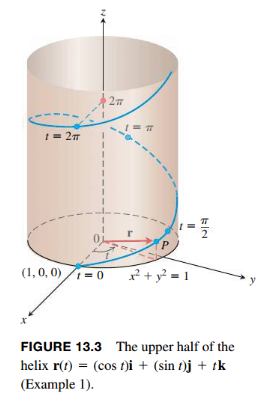
\includegraphics[width = 0.35\textwidth]{vvf1.png}
\end{center}

\begin{remark*}[2]
  (Taken from Practice Midterm D) Let $ C $ be
  a conic in $ \R^{3}$ defined by the following
  system of equations:
  \[ \frac{(x-1)^{2}}{9} + \frac{(z-2)^{2}}{25} = 1\]
  \[ y = 3 \]
  \begin{enumerate}
    \item Describe $ C $ qualitatively: include
          what type of conic it is, what its center
          is, and how it is situated in $ \R^{3} $.
    \item Give a vector parameterization $ r(t)$
          for $ C$. Include explicit bounds
          $ a \leq t \leq b $ ensuring that
          the entire curve is parameterized.
  \end{enumerate}

\end{remark*}

\section{Parametric Equations of Conic Sections}%
\label{sec:label}
We are able to actually generate functions
of geometric shapes using parametric equations.
Sure, we know that shapes such as circles, ellipses,
and hyperbolas are defined by the following equations,
respectively
\[ x^{2} + y^{2} = c^{2}\]
\[ \frac{(x-h)^{2}}{a^{2}}+\frac{(y-k)^{2}}{b^{2}} = 1^{2}\]
\[ \frac{(x-h)^{2}}{a^{2}}-\frac{(y-k)^{2}}{b^{2}} = 1^{2}\]

But these aren't \textbf{functions}, as the movement of
x, for example, isn't going to affect the movement in the
y or the z direction. Therefore, how are we able
to actually rewrite these familiar geomtetric formulas
as \textbf{parametric equations?}
\begin{itemize}
  \item We represent the movement of each
        dimension as through
        \textbf{polar coordinates}.
  \item Functions with polar coordinates
        generally just have some constant
        that represents the ``radius'' $ r $,
        but are all dependent on the
        angle $ \theta $. Therefore,
        if we rewrite everything as a
        polar coordinate function, then
        we can thereby make a
        \textbf{parametric equation
        of any geometric shape}.
\end{itemize}

\subsection{Parametric Equation of a Circle}
\begin{center}
  \fbox{
    \parbox{\textwidth} {
      \begin{definition}
        Parametric Form of a Circle
      \end{definition}
      \textbf{Recall.}
      \\
      The standard form of a circle
      is given by the equation
      \[ (x-h)^{2} + (y-k)^{2} = r^{2}\]
      Movement in the x and y direction
      in polar coordinate form
      is defined by the following
      equations, where $ r $ represents
      the \textbf{magnitude or radius}.
      \[ x = r\cos{t}; y = r\sin{t}\]
      \textbf{Formula.} \\
      Therefore, the parametric
      form of a circle must be
      \[ F(t) = \langle x(t), y(t) \rangle\]
      \[ \langle r\cos{t} + h,   r\sin{t} + k\rangle \]
    }
  }
\end{center}

\subsection{Parametric Equations of Ellipses}
\begin{center}
      \dfn{Parametric Form of an Ellipse}

      {\textbf{Recall.}
      \\
      The standard form of an ellipse is
      defined by the following characteristics
      \begin{enumerate}
        \item Both terms of equation are positive
      \end{enumerate}

      \[ \frac{(x-h)^{2}}{a^{2}} + \frac{(y-k)^{2}}{b^{2}} = 1 \]

      Additionally, we can remember our
      simple polar coordinate formulas
      \[ x = r\cos{\theta}; y = r\sin{\theta}; \tan{\theta} = \frac{y}{x}\]
      We can think of the the $ h $ and the $ k $ values
      as \textbf{offsets} to the sine and cosine functions. \\
      \textbf{Formula.} \\
      If we make the proper substitutions, we are
      able to arrive at the following formula
      \[ F(t) = \langle x(t), y(t) \rangle\]
      \[ x(t) = a\cos{t} + h\]
      \[ y(t) = b\sin{t} + k \]
    }
  \end{center}

\subsection{Parametric Equations of Hyperbolas}
\begin{center}
  \fbox{
    \parbox{\textwidth} {
      \begin{definition}
        Parametric Form of a Horizontal Hyperbola
      \end{definition}
      \textbf{Recall.} \\
      The standard form of a hyperbola
      is defined by the following characteristics
      \begin{enumerate}
        \item Both terms are of unlike signs, ie:
              one is positive and the other is negative
      \end{enumerate}
      and is given by the following equations:
      \[ \frac{(x-h)^{2}}{a^{2}} - \frac{(y-k)^{2}}{b^{2}} = 1 \]
      \textbf{Formula.}
      Instead of utilizing the sine and cosine
      functions, however, the hyperbola utilizes
      parametric equations based off of
      functions of \textbf{secant} and
      \textbf{tangent}, where positive terms
      are functions of \textbf{secant} and
      negative terms are functions of \textbf{tangent.}
      The horizontal formula of a hyperbola is
      as follows
      \[ F(t) = \langle x(t), y(t) \rangle\]
      \[ x(t) = a \sec{\theta} + h \]
      \[ y(t) = b \tan{\theta} + k \]

    }
  }
\end{center}

\begin{center}
  \fbox{
    \parbox{\textwidth} {
      \begin{definition}
        Parametric Form of a Vertical Hyperbola
      \end{definition}
      \textbf{Recall.} \\
      The standard form of a hyperbola
      is defined by the following characteristics
      \begin{enumerate}
        \item Both terms are of unlike signs, ie:
              one is positive and the other is negative
      \end{enumerate}
      and is given by the following equations:
      \[ \frac{(y-k)^{2}}{a^{2}} - \frac{(x-h)^{2}}{b^{2}} = 1 \]
      \textbf{Formula.}
      Instead of utilizing the sine and cosine
      functions, however, the hyperbola utilizes
      parametric equations based off of
      functions of \textbf{secant} and
      \textbf{tangent}, where the positive term
      always gets the \textbf{secant function}
      and the negative terms always gets \textbf{tangent.}


      The parametric equation of a vertical hyperbola is
      as follows
      \[ F(t) = \langle x(t), y(t) \rangle\]
      \[ x(t) = b \tan{\theta} + h \]
      \[ y(t) = a \sec{\theta} + k \]

    }
  }
\end{center}


\subsection{Parametric Equations of Parabolas}
\begin{center}
  \fbox{
    \parbox{\textwidth} {
      \begin{definition}
        Parametric Form of a Parabola
      \end{definition}
      \textbf{Recall.} \\
      The standard form of a parabola
      possesses the following characteristics
      \begin{enumerate}
        \item One variable is squared and the
              other variable is not
      \end{enumerate}
      and is given by the following equations:
      \[ y^{2} = 4ax ~ \textrm{for a horizontal parabola}\]
      \[ \textrm{or}\]

      \[ x^{2} = 4ay ~ \textrm{for a vertical parabola}\]
      \textbf{Formula.}
    }
  }
\end{center}

\section{Limits and Continuity}
Now that we have essentially learned all
of the basic operations of vectors,
as well as have evaluated functions
that return vectors, let us try to
apply concepts from \textbf{calculus}
to these functions.
\par Recall that the limit of a function
essentially states that there exists
some number $ \delta $, at which
every value of the function for
all values of the domain greater than
$ \delta $ will possess a corresponding
$ \varepsilon $ distance from the limit.
\par Essentially, we know that a limit
basically states that if the domain
of a function gets aribtrariliy close
to some value $ a $, then the value of the
function must approach some value $ L $.

\begin{center}
  \fbox{
    \parbox{\textwidth} {
      \begin{definition}
        Limits of a Vector-Valued Function
      \end{definition}
      The limit $ \lim_{t \to a} \vec{r}(t) $
      exists and equals $ \vec{s} = \langle
      s_{1}, s_{2}, s_{3} \rangle$
      if and only if
      \[ \lim_{t \to a}f(t) = s_{1}, \lim_{t \to a} g(t)= s_{2},
      \lim_{t \to a} h(t) = s_{3}\]
    }
  }
\end{center}

\begin{center}
  \fbox{
    \parbox{\textwidth} {
      \begin{definition}
        Continuity of a Vector-Valued Function at a Point
      \end{definition}
      A vector-valued function $ \vec{r}(t) $ is \textbf{continuous}
      at a point $ t_{0}$ if $ f(t)$, $g(t)$, and $h(t)$ are
      continuous at $ t_{0}$ or
      \[ \lim_{t \to t_{0}}f(t) = f(t_{0}), \lim_{t \to t_{0}}g(t) =
      g(t_{0}), \lim_{t \to t_{0}}h(t) = h(t_{0}) \]
    }
  }
\end{center}

\begin{center}
  \fbox{
    \parbox{\textwidth} {
      \begin{definition}
        Contunity of a Vector-Valued Function as as Function
      \end{definition}
      The vector-valued function $ \vec{r}(t)$
      is continuous as a function if $ \vec{r}(t)$
      is continuous at \textbf{every point}  in its domain.
    }
  }
\end{center}

\section{Derivatives of Vector-Valued Functions}
Similarly to how we evaluated the limits of
\textbf{vector-valued functions}, we can also
evaluate the \textbf{derivatives of vector-valued}
functions in a similar manner.
\par Much like limits, we evaluate derivatives
of \textbf{vector-valued functions} by
evaluating the derivatives of each
\textbf{component function}.

\begin{center}
  \fbox{
    \parbox{\textwidth} {
      \begin{definition}
        Derivatives of Vector-Valued Functions
      \end{definition}
      The vector function $ r(t) = f(t)\hat{i} + g(t)\hat{j} +
      h(t)\hat{k}$ has a derivative (or is differentiable) at
      $ t $ if and only if $ f$, $g$, and $ h $ have
      derivatives at $ t $. Then, the derivative of the
      vector function is equal to
      \[ r'(t) = \frac{d}{dt}r =
        \lim_{\triangle \to 0}\frac{r(t + \triangle{t}) - r(t)}{\triangle{t}}
      \]
      \[ \Rightarrow \frac{df}{dt}\hat{i} +
        \frac{dg}{dt}\hat{j} +
        \frac{dh}{dt}\hat{k} \]
      \[ \Rightarrow \langle \frac{df }{dt},
        \frac{dg}{dt}, \frac{dh}{dt}\rangle\]
    }
  }
\end{center}
\begin{remark*}[(1)]

\end{remark*}

\subsection{Understanding Derivatives of Vector-Valued
  Functions}
\begin{center}
  \fbox{
    \parbox{\textwidth} {
      \begin{definition}
        Vector-Valued Functions in Particle Motion
      \end{definition}
      If $ r $ is the position vector of a particle
      moving along a smooth curve in space, then
      \[ v(t) = \frac{dr}{dt} = r'(t)\]
      is the particle's $ velocity vector $, which
      is the vector that is tangent to the curve.
      At any time $ t $, the direction of $ v $
      is known as the \textbf{direction of motion},
      while the magnitude of $v $ is the
      particle's \textbf{speed}, and the derivative
      \[ a = \frac{dv}{dt} = v'(t) = r''(t)\]
      is the particle's \textbf{acceleration vector}.
      \begin{enumerate}
        \item Velocity $ v(t)$ is the derivative
              of position $ r(t)$
        \item Speed is the magnitude of velocity
              $ || v(t) || $
        \item Accleration $ a(t)$ is the derivative
              of velocity $ \frac{dv}{dt} = \frac{d^{2}r}{dt^{2}}$
        \item The unit vector $ \frac{v}{||v||}$ is the
              direction of motion at time $ r $.

      \end{enumerate}

    }
  }
\end{center}

\begin{remark*}[(4)]
  Find the velocity, speed, and
  accleration of a particle whose
  motion in space is given by the
  position vector
  \[ r(t) = 2\cos{t}\hat{i} + 2\sin{t}\hat{j} +
    5\cos^{2}{t}\hat{k}\]
  Sketch the velocity vector of $ v(\frac{7\pi}{4})$
\end{remark*}
\section{Differentiation Rules for Vector-Valued Functions}
\begin{center}
  \fbox{
    \parbox{\textwidth} {
      \begin{definition}
        Differentation Rules of Vector-Valued Functions
      \end{definition}
      \begin{enumerate}
        \item Constant Function Rule
        \item Scalar Multiple Rule
        \item Sum Rule
        \item Difference Rule
        \item Dot Product Rule
        \item Cross Product Rule
        \item Chain Rule

      \end{enumerate}

    }
  }
\end{center}
\section{Integrals of Vector-Valued Functions}
TODO
\subsection{Understanding Integrals of Vector-Valued
  Functions}
TODO

% Chapter 13.3: Arc Length
\chapter{13.3: Arc Length}
\section{Reminders}
\section{Objectives}
\section{Motivation}
\chapter{14.1: Functions of Several Variables}
\section{Reminders}
\section{Objectives}
\section{Motivation}
\chapter{14.3: Partial Derivatives}
\section{Reminders}
\section{Objectives}
\section{Motivation}
\chapter{14.4: The Chain Rule}
\section{Reminders}
\section{Objectives}
\section{Motivation}
\chapter{14.5: Gradient Vectors and Tangent Planes}
\section{Reminders (As of 05/20/23)}
\subsection{MATH\_226}
\subsection{MATH\_230}
\section{Objectives}
\section{Motivation}
\chapter{14.5 (cont'd): Directional Derivatives}
\section{Reminders}
\subsection{MATH\_226}
\subsection{MATH\_230}
\section{Objectives}
\section{Motivation}
\chapter{14.6: Tangent Planes and Linearization}
\section{Reminders}
\subsection{MATH\_226}
\subsection{MATH\_230}
\section{Objectives}
\section{Motivation}
\section{Review: Finding the Tangent Line to a Curve}
\ex{Review: Find Tangent Line ot a Curve}{
  Find the tangent line to the curve
  \[ \frac{x^{2}}{9} + y^{2} = 1 \]
  at the point $(0,1)$}
\sol
In single variable calculus, we would consider
two different techniques:
\begin{itemize}
  \item Solving for $ y $, then solving for $ y'(0) $
  \item Implicit differentiation (which is
        evaluating $\frac{dy}{dx}$ in terms of $ y $)
\end{itemize}

In multivariable calculus, however, we take a
different approach:
\begin{itemize}
  \item We think of the function as a level curve of
        $ f(x,y) = z $. The \textbf{gradient
        vector} of the function at that point
        will be perpendicular to the level curve.
\end{itemize}

\nt{A gradient
  vector is given by the following form
  \[ \nabla f(x,y) = \left( \frac{\partial f}{\partial x} \frac{\partial f}{\partial y}\right)\]}

\[ f(x,y) = \frac{x^{2}}{9} + y^{2}\]
\[ \nabla f(x,y) = \left( \frac{\partial}{\partial x} \left( \frac{x^{2}}{9} + y^{2} \right),
    \frac{\partial}{\partial y} \left( \frac{x^{2}}{9} + y^{2} \right)\right)\]
\[ \Rightarrow \nabla f(x,y) = \left( \left( \frac{2x}{9} \right),
    \left( 2y \right) \right)\]
\[ \Rightarrow \nabla f(x,y) ~\Big |_{(0,1)} =
  \left( \left( \frac{2(0)}{9} \right), \left( 2(1) \right) \right) = \left( 0,2 \right) = \nabla f(x,y)\]
Therefore, we know that the equation of the
tangent line is given by
\[ Ax + By = C \]
\[ \Rightarrow F_{x}(x-h) + F_{y}(y-k) = 0 \]
\[ \Rightarrow 0 \left( x-0 \right) + 2 \left( y-1 \right) = 0 \]
\[ \Rightarrow y = 1 \]
\nt{In order to find the tangent line to a given
  shape (in the former case, an ellipse), all we have
  to do is just find the \textbf{gradient vector} at
  the given point, then substitute the proper values in.}

But what if we want to find the tangent \textit{something} for a function with more than
two variables?

\section{Finding Tangent Planes}
In the former example, we were working with
exclusively two variables in $ \R^{2}$, but what
if we wanted to translate these techniques into
$ \R^{3}$?
\par Well, it is first important to remember
that in three dimensions, we are working with surfaces,
which means that if we were to find the tangent-\textit{something} to a surface, we would be able
to extend it in some third direction.
\begin{center}
  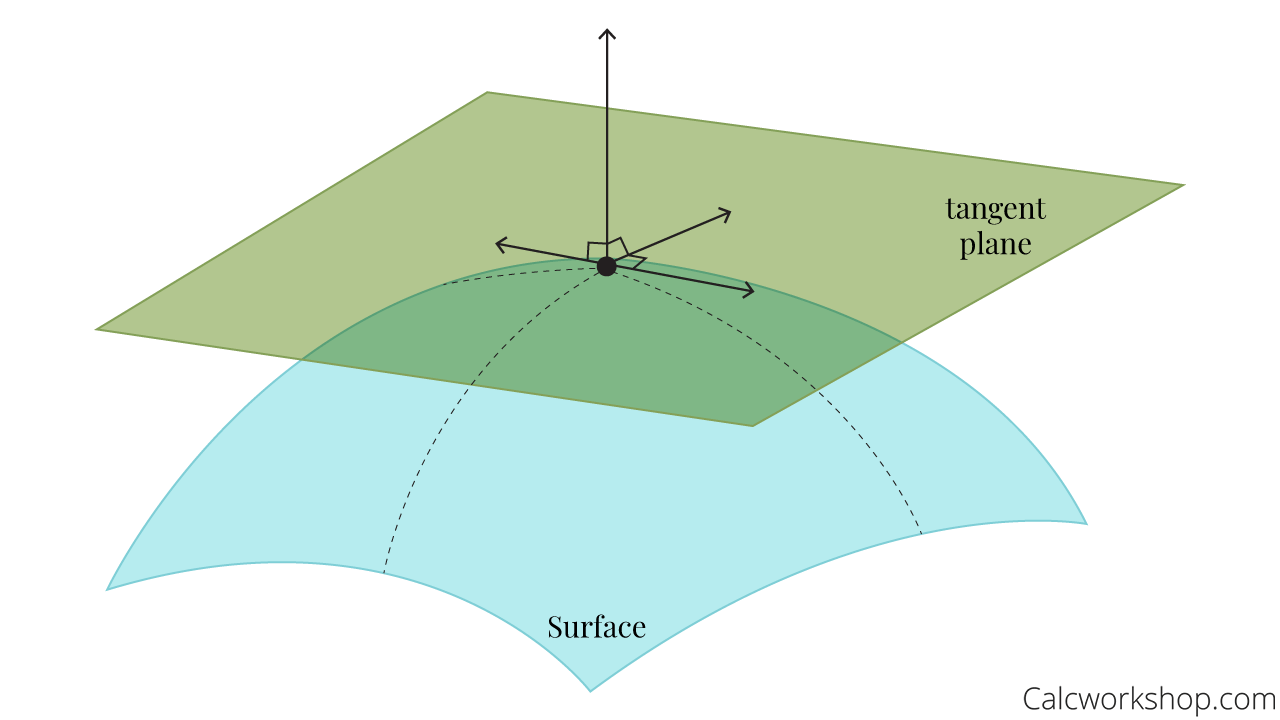
\includegraphics[width = 0.5 \textwidth]{tan1.png} \\
  \caption{Notice how \textit{all} of the values
    in the plane are tangent/perpendicular to the
  surface\dots}
\end{center}
All of this culminates in the idea that, whenever
we are working with a function of \textbf{three variables,} we are now working with not just a tangent line, but a tangent \textit{plane}. If we wanted
to evaluate the equation of this tangent plane,
we apply the same general concept for finding
the equation of the tangent line in $ \R^{2} $.

\ex{Finding a Tangent \textit{Plane}}{
  Find the tangent plane to
  \[ \frac{x^{2}}{9} - \frac{y^{2}}{16} +
    \frac{z^{2}}{25} = 1 \]
  at the point $ (3,4,5 )$}.

Much like in the previous example, we apply
our understanding of gradients to
finding the tangent plane.

\nt{It is important to our understanding that
  the gradient represents the movement of the
  function in terms of \textit{each of its variables}.
  The gradient in this case is effectively
  the derivative of a function in single-varialbe
  calculus. Although there are multiple
  rates of change within a multivariable function and
  a surface, the gradient represents the \textbf{best
    possible direction that represents the ``slope''.}}
Anyways, the algorihtm for evaluating the tangent plane is just like evaluating the tangent line.
\begin{itemize}
  \item We first evaluate the \textbf{gradient vector} of the function $f(x,y,z)$
  \item Then, we just plug the point at which
        we want to find the ``slope''of into
        the gradient
  \item Finally, we want to apply the
        value of the gradient at a point as well
        as the original point into the standard
        formula of a plane.
\end{itemize}

\[ \nabla f(x,y,z) = \left( \frac{\partial f}{\partial x}, \frac{\partial f}{\partial y}, \frac{\partial f}{\partial z } \right)\]
\[ \Rightarrow \nabla f(x,y,z) = \left( \frac{\partial }{\partial x} \left( \frac{x^{2}}{9} - \frac{y^{2}}{16} + \frac{z^{2}}{25} -1 \right), \frac{\partial }{\partial y}\left( \frac{x^{2}}{9} - \frac{y^{2}}{16} + \frac{z^{2}}{25} -1 \right), \frac{\partial }{\partial z }\left( \frac{x^{2}}{9} - \frac{y^{2}}{16} + \frac{z^{2}}{25} -1 \right) \right)\]
\[ \Rightarrow \nabla f(x,y,z) = \left( \frac{2x}{9}, \frac{-2y}{16}, \frac{2z}{25} \right)\]
\[ \Rightarrow \nabla f(x,y,z) \Biggr|_{(3,4,5)}
  = \left( \frac{2(3)}{9}, \frac{-2(4)}{16},
    \frac{2(5)}{25} \right)\]
\[ \Rightarrow \nabla f(x,y,z) = \left( \frac{2}{3}, \frac{-1}{2}, \frac{2}{5} \right)\]

\nt{Recall that the equation of a
  plane is given by
  \[ A(x-x_{0}) + B(y-y_{0})+ C (z-z_{0}) = 0 \]}

  \[ A(x-x_{0}) + B(y-y_{0})+ C (z-z_{0}) = 0 \]
  \[ \Rightarrow \frac{2}{3}(x-3) + \frac{-1}{2}(y-4) +
    \frac{2}{5}(z-5) = 0 \]

\section{Summary of Evaluating Tangent-\textit{somethings}}
  \dfn{How to Evaluate a Tangent Line to a Level Curve}{Given a level curve $f(x,y) = c$,
    we are able to find the \textbf{tangent line} at
    $ (a,b) $ by evaluating
    \begin{equation}
      f_{x}(a,b) (x-a) + f_{y}(a,b)(y-b) = 0\label{eq1}
    \end{equation}

    It is important to remember, though, that the
    general methodology to achieve \eqref{eq1} is
    the following:
    \begin{enumerate}
      \item Evaluate the gradient vector of the
            levle curve $ \nabla f(x,y) $
      \item Evaluate the value of the gradient
            vector at the given point $ (a,b)$
      \item Plug hte vlaues into the
            standard equatoin of a line
            \[ Ax + By = C \]
    \end{enumerate}

  }

  \dfn{How to Evaluate a Tangent Plane}{
    Given a level surface $f(x,y,z) = d$, we
    can find the \textbf{tangent plane} to the surface
    at a point $ (a,b,c)$ by evaluating
    \begin{equation}
      f_{x}(a,b,c)(x-a) + f_{y}(a,b,c)(y-b) +
      f_{z}(a,b,c)(z-c)= 0 \label{tan2}
    \end{equation}
    In order to achieve the equation \eqref{tan2},
    you can also follow the algorithm:
    \begin{enumerate}
      \item Evaluate the \textbf{gradient vector} of
            the level curve $ \nabla f(x,y,z)$
      \item Evaluate the value of the
            gradient vector at the given point $ (a,b,c)$
      \item Plug the values of the gradient
            vector at a point as well as the given point
            into the standard form of a plane
            \[ A(x-x_{0}) + B(y-y_{0}) + C(z-z_{0}) = 0 \]
    \end{enumerate}

}

\section{Linearization in Single and Multivariable Calculus}
In this next section, we are discussing \textbf{linearization of functions}, which should
recall the idea of the \textbf{Taylor Series}.
\begin{itemize}
  \item Recall that the Taylor Series is an infinite
        sum representation of a function (also known
        as the generating function). What makes
        the Taylor Series special is that we are
        able to derive this infinite sum representation
        by \textbf{only using the function itself}.
        The Taylor series is created by
        using a function and its derivatives. The
        more terms that we add to the Taylor Polynomial,
        the more accurate that the approximation is.
        The point at which the Taylor Series converges
        is the function itself (or at least, very
        close).
\end{itemize}

\nt{The Taylor Series of a function $ f(x) $ at
  some center of convergence $ a $ is given
  by the infinite sum:
  \[ \sum_{n=0}^{\infty} \frac{f^{(n)}(a)}{n!}(x-a)^{n} \]
  which translates to
  \[ \Rightarrow f(a) + \frac{f'(a)}{1!}(x-a) + \frac{f''(a)}{2!}(x-a)^{2} + \frac{f^{(3)}(a)}{3!}(x-a)^{3} + \cdots +
    \frac{f^{(n)}(a)}{n!}(x-a)^{n}\]
}

``Linearization'' is just another name for the
\textbf{first-order Taylor expansion}. So,
whenever we are evaluating the linearization of a
function, we are essentially just finding the
\textbf{first-order Taylor expansion} of the function,
the terms of hte Taylor expansion up until the
first derivative of the function, inclusive.

\par Let us first recall what linearization looks like
in single variable calculus\dots

\dfn{Linearization (Single Variable Calculus)}{
  The linearization of a function $ y = f(x)$ at some
  center $ x = a $ is equal to

  \[ y = f(a) + \frac{f'(a)}{1!}(x-a)\]
which we can also denote as
\[ L(x) = f(a) + \frac{f'(a)}{1!}(x-a)\]
such that $ L(x)$ is just the linearization of
the function $f(x)$. }


\subsection{Linearization in Multivariable Calculus}
\dfn{Linearization (Multivariable Calculus)}{
  The linearization of $ z = f(x,y)$ at a point
  $(a,b)$ is
  \begin{equation}
    f(a,b) + f_{x}(a,b)(x-a) + f_{y}(a,b)(y-b)\label{tan3}
  \end{equation}
  Notice that this equation is also the same as
  \begin{equation}
    L(x,y) = f(a, b) + \frac{\partial f}{\partial x}(x-a) +
    \frac{\partial f}{\partial y}(y-b)
  \end{equation}
  such that $ f(a,b)$ is current value of the function
  at a point, $ f_{x}(a,b)(x-a)$ is the partial
  derivative of the function with respect to $ x $
  and $ f_{y}(a,b)(y-b)$is the partial derivative
  of the function with respect to $ y $. \\ \\
  \textbf{Intuition.} \\
  Our intuition here is that we are finding
  the equation of the plane that is tangent
  to the surface at the given pint, and then
  we are solving for the z term.
}

\ex{Multivariable Linearization Example 1}{
  What's bigger: $\sqrt{9.1}$ or $\sqrt{27.2}$?}

\sol Since we are unable to actually compute
the values of $\sqrt{9.1}$ and $\sqrt[3]{27.2}$, we
can use \textbf{linearizaiton} in order to approximate
the difference between $\sqrt{9.1}$ and $\sqrt{27.2}$.
\par We can use the following equation to evaluate
the difference between $ \sqrt{9.1}$ and $\sqrt{27.2}$
\[ f(x,y) = \sqrt{x} - \sqrt[3]{y} \]
and we will center our approximation at the point
\[ (a,b) = (9, 27) \]
since it is reasonably close to what we are
trying to approximate.

\nt{Remember that the first-order Taylor expansion of a multivariable
  function is given by the following function
  \begin{equation}
    P_{1}(x,y) = f(a,b) + f_{x}(a,b)(x-a) + f_{y}(a,b)(y-b)
  \end{equation}

}
In order to evaluate $f_{x}$ and $ f_{y}$, let us
just evaluate the \textbf{gradient vector} of
$ f(x,y)$ and then work with the components
of the gradient vector.

\[ \nabla f(x,y) = \left( f_{x}, f_{y} \right)\]
\[ \Rightarrow \nabla f(x,y) = \left( \frac{\partial}{\partial x} \left( \sqrt{x} -
      \sqrt[3]{y} \right), \frac{\partial}{\partial y}
    \left( \sqrt{x} - \sqrt[3]{y} \right)\right)\]
\[ \Rightarrow \nabla f(x,y) =
  \left( \frac{1}{2}x^{-\frac{1}{2}},
    \frac{1}{3}y^{-\frac{2}{3}}\right)\]
\[ \Rightarrow f_{x} = \frac{1}{2}x^{-\frac{1}{2}},
  f_{y} = -\frac{1}{3}y^{-\frac{2}{3}}\]
Now, the linearization equation is as follows:
\[ L(x,y) = f(a,b) + f_{x}(a,b)(x-a) + f_{y}(a,b)(y-b)\]
\[ \Rightarrow = f(9,27) + \frac{1}{2}9^{-\frac{1}{2}}(x-9) - \frac{1}{3}27^{-\frac{2}{3}}(y-27) \]
\[ \Rightarrow = (0) + (\frac{1}{6})(x-9) - \frac{1}{27}(y-27)\]
Now, we can just substitute our original values
$x = 9.1$ and $ y = 27.2$
\[ \rightarrow \left( \frac{1}{6} (9.1-9) \right)
  - \left( \frac{1}{27} \right) (27.2-27) \]
\[ \Rightarrow \left( \frac{1}{6} \right) (0.1) +
  \left( \frac{1}{27} \right) (0.2) \]
\[ \Rightarrow L(x) > 0 \]
Now that's cool that we were able to find this
value, but how can we actually be sure that
we are correct? How can we be sure that our
approximation didn't give us the wrong number? After
all, it's possible that perhaps $\sqrt{9.1}$ is
much smaller than we assumed it was, which would
yield a \textbf{negative value} for $L(x)$,
indicating that $\sqrt{9.1}$ is smaller. \\ \\
Fortunately, there is a way for us to actually
calculate \textit{the interval with which our
approximation is actually correct}.
\section{Taylor's Formula (Separating Approximation from Error)}
From Calculus 2 (or just Sequences and Series),
we remember that Taylor actually accounts for
the difference between the approximation of a
finite Taylor Polynomial at a point and the actual
value of a function at that same point. He essentially
states that the Taylor Series $T(x) $(that is, the infinite
sum), will always be composed of two parts:
\begin{itemize}
  \item A finite polynomial approximation of the
        Taylor Expansion $ P_{n}(x)$
  \item The difference between the finite Taylor
        polynomial at a point
        and the actual value of the functoin
        at that point, the remainder $ R_{n}(x)$

\end{itemize}
such that $ n $ represents the order of the Taylor
Polynomial.
\[ T(x) = P_{n}(x) + R_{n}(x)\]

\dfn{Taylor Error Estimation Theorem (Or Lagrange
  Estimation Theorem)}{
  Given that a  functoin $ z = f(x,y)$ and all of its
  partial derivatives $ f_{x}, f_{y}, f_{xx}, f_{xy}, f_{yy}$
  are all \textit{continuous} at and near a point $ (a,b)$. We know that the \textbf{next terms of the
    Taylor expansion}, given by the coefficients
  $ |f_{xx}|, |f_{yy}|, |f_{xy}|$ will be, at most, some
  constant $ M $. Therefore, the remainder $ R_{n} $
  for the 1st Taylor expansion of a multivariable
  functoin is given by
  \begin{equation}
    R_{1}(x) = \left| f(x,y) - L(x,y) \right| \le
    \frac{1}{2!}M(\left| x-a \right| + \left| y-b \right|)^{2} \label{error}
  \end{equation}
  It is important to remember that \eqref{error}
  represents the \textit{maximum possible value}
  that the next term in the Taylor expansion can be.
  Remember that the second Taylor expansion of a
  multivariable function will include terms
  that have coefficients of mixed partial derivatives
  $ \left| f_{xx} \right|, \left| f_{xy} \right|, \left| f_{yy} \right|$. The only thing that we are doing
  is that we are calculating this ``worst case scenario'', in which all of these terms have the highest possible coefficient, which is one of those
  second-order partial derivatives.
}
\nt{The error bound is \textit{not} meant to be accurate, but rather, a \textbf{doomsday marker}. }
\ex{Applying the Taylor Estimation Theorem to the Previous Example}{Given a
  function
  \[ f(x,y) = \sqrt{x} - \sqrt[3]{y}\]
that is linearized at the center $ (a,b) =  (9,27)$,
find the error bound of the linearization at
the point $ (9.1, 27.2)$.}
\sol TODO
\chapter{10.9: Taylor Polynomials}
\section{Reminders}
\section{Objectives}
\section{Motivation}
\section{Review of Single Variable Taylor Polynomials}
\ex{Review Taylor Polynomials}{
Given a generating function $ f(x) = e^{x}$, we
are able to approximate the value of this generating
function with the following $n$th order Taylor polynomials. Let us find the Taylor Polynomials
of $ f(x)$ near the center $ a = 0 $}
\nt{A Taylor Polynomial is a \textit{truncated} version
  of a Taylor Series. The $n$th order Taylor polynomial
  just represents the terms up until the term with the
  $n$th order derivative as its coefficient. The
  Taylor Series is given by the infinite sum
  \[ \sum_{n=0}^{\infty} \frac{f^{(n)}(a)}{n!}(x-a)^{n}\]
  \[ \Rightarrow f(a) + \frac{f'(a)}{1!}(x-a) +
    \frac{f''(a)}{2!}(x-a)^{2} + \frac{f^{(3)}(a)}{3!}(x-a)^{3} + \cdots +
  \frac{f^{(n)}(a)}{n!}\]}
\sol
\[ T_{0}(0) = e^{0} \Rightarrow 1 \]
\[ T_{1}(0) = e^{0} + \frac{e^{0}}{1!}x \Rightarrow 1 + \frac{1}{1!}x\]
\[ T_{2}(0) = e^{0} + \frac{e^{0}}{1!}x + \frac{e^{0}}{2!}x^{2} \Rightarrow 1 + \frac{1}{1!}x +
\frac{1}{2!}x^{2}\]
\[ T_{3}(0) = e^{0} + \frac{e^{0}}{1!}x +
  \frac{e^{0}}{2!}x^{2} + \frac{e^{0}}{3!}x^{3}
\Rightarrow 1 + \frac{1}{1!}x +
\frac{1}{2!}x^{2} + \frac{1}{3!}x^{3} \]
From this, we know that the Taylor Series, based
on the pattern of the terms in the Taylor Polynomials
is given by the following summation:
\[ \sum_{n=0}^{\infty} \frac{1}{n!}x^{n} \]
\nt{It is ipmortant to remember that the higher
  the order of the Taylor Polynomial $\rightarrow$
  the more accurate (and therefore the less the remainder) that the Taylor Polynomial will have. }
Again, it is important to remember that this entire idea
of Taylor Polynomials and Remainders is all given
by the \textbf{Taylor Theorem}.
\dfn{Taylor Theorem (Single Variable)}{
  If $ f $ is $ n $ times differentiable at $ x = 0 $,
  then $ \left| f(x) - P_{n}(x) \right| \cdot \frac{1}{x^{n}} $ will approach zero. That is, if a
  function is infinitely differentiable, then the higher order the Taylor Polynomial $ P_{n}(x)$ is,
  the less difference between the Taylor Polynomial
  and the generating function $ f(x)$.
  \par From this, the error $R_{n}$ for
  the $n$th Taylor Polynomial centered at
  $ a = 0 $is given by the
  following equation:
  \begin{equation}
    R_{n}(x) = \left| f(x_{0}) - P_{n}(x_{0}) \right|
    \le \frac{1}{(n+1)!}M \left| x_{0} \right|^{n+1} \label{remainder}
  \end{equation}}
such that $ M $ is the maximum possible Taylor
coefficient $ f^{(n+1)}(x) $ between $ -x_{0} $ and
$ x_{0}$.
We can of course, actually apply this same
principle to \textbf{multivariable functions}, the
only caveat is that, as we add more terms to the
Taylor polynomial, the more complex the
equation is going to be.
\begin{itemize}
  \item We are no longer just finding the
        second, third, or $n$th derivatives,
        but because we are working with multivariables,
        we have to also account for the repeating
        partial derivatives, such as $ f_{xx} $ and
        $ f_{yy}$ as well as \textbf{mixed partial
        derivatives} such as $ f_{xy}$
\end{itemize}

\section{Why use higher-order Taylor Polynomials?}
The reason why we would even consider caring
about these higher order (and more complex)
Taylor Polynomials is that, as we add more terms,
the more context we have on the behavior of the graph.
\begin{itemize}
  \item We can think of adding more Taylor terms
        as adding more ``hills'' and ``valleys''
  \item We can also think of the fact that
        the $n$th order derivatives of a function
        reveal more information about their
        graphical behavior.
\end{itemize}
So, what can $ z = P_{2}(x,y)$ detect about
the behavior of a function $ f(x,y)$ that the
first-order Taylor polynomial $ z = P_{1}(x,y)$ cannot?
\begin{itemize}
  \item \textbf{First-order Taylor polynomials} $P_{1}(x) \rightarrow$ Increasing/Decreasing behavior
  \item \textbf{Second-order Taylor polynomials} $P_{2}(x) \rightarrow$ Concavity behavior
\end{itemize}
\ex{Multivariable Second-Order Taylor Polynomials}{
  Given the function
  \[ f(x,y) = e^{x+y} + y^{2}\]
  Find the second-order Taylor polynomial $ P_{2}(x,y)$
  about the center point $(0,0)$. }
\sol TODO

\dfn{Multivariable Error Estimation Theorem}{
  The remainder of a multivariable $n$th order
  Taylor polynomial $R_{n}$ is given by the following expression
  \begin{equation}
    R_{n}(x) \le \frac{1}{(n+1)!} M_{n+1}
    \left( \left| x-a \right| + \left| y-b \right|\right)^{n+1} \label{multi-error}
  \end{equation}

}

\nt{We now have a subscript for $ M$, since we have
  to remember that $ M$, unlike in single variable
  calculus, does not consist of a single possible value
  (that is, the next derivative), instead
  we have to consider \textit{all possible coefficients}
  and combinations of the $n$th order partial derivatives
  of a function. }
\ex{Error Bound of Multivariable Taylor Polynomial}{}
\chapter{14.6: Extreme Values and Saddle Points}
\section{Reminders}
\section{MATH\_226}
\begin{itemize}
  \item written homework due friday
        \item final exam is in \textit{13 days}

\end{itemize}

\section{MATH\_230}
\begin{itemize}
  \item written homework due tonight
  \item mylab math 17: extreme values and saddle points is due tomorrow
  \item exam is in \textit{12 days}
\end{itemize}

\section{Objectives}
\section{Motivation}
\section{Recapping Important Terminology}
Over the last few sections, we have discussed
some pretty useful concpets and ideas, including
\begin{itemize}
  \item partial derivatives
  \item gradient vectors
  \item directional derivatives
\end{itemize}

\dfn{Gradient Vectors}{Given a function $ z = f(x,y)$, the gradient of f(x,y) is equal to
  \[ \nabla f(x,y) = ( f_{x}(x,y), f_{y}(x,y) ) \]
  The gradient represents a data type that \textit{stores} all first derivatives of a given function.}
Along the same train of thought, we also have the concept of the \textbf{Hessian Matrix}.
\dfn{Hessian Matrix}{Given a function $ z = f(x,y)$, the Hessian of $f(x,y)$ is equal to the 2x2 matrix
  \[ Hf(x,y) = Hess(f)(x,y) = \]
  \begin{center}
  \begin{bmatrix}
    f_{xx}(x,y) & f_{xy}(x,y) \\
    f_{yx}(x,y) & f_{yy}(x,y) \\
  \end{bmatrix}
  \end{center}
  which, of course, is just a data type that
  stores all of the second-order and second-order mixed partial derivatives of a function $ f $.

}
\subsection{More About Matrices}
\dfn{Diagonals of Matrices}{In the following diagram, we observe the \textbf{main diagonal} as well as the \textbf{off diagonal} of a matrix. The easiest way to remember these is that the main diagonal is going from \textit{left to right} whereas the off diagonal is going from \textit{right to left}.

  \begin{center}
    Given the 2x2 matrix:
    \begin{bmatrix}
      a & b \\
      c & d \\
    \end{bmatrix},

    the \textbf{main diagonal} is as follows:
    \begin{bmatrix}
      a & {} \\
      {} & d \\
    \end{bmatrix},

    whereas the \textbf{off diagonal} is as follows:
    \begin{bmatrix}
      {} & b \\
      c & {} \\
    \end{bmatrix}


  \end{center}}


\dfn{Determinants}{The determinant of a 2x2 matrix is equated by finding the difference between the product of the main diagonal terms as well as the product of the terms in the off diagonal. \textbf{Warning:} this formula only applies for \textit{2x2 matrices} and does \textit{not} apply to larger matrices.

  \begin{center}
    \textit{det}
    \begin{pmatrix}
         a & b \\
         c & d \\
    \end{pmatrix}
    \[ = a \cdot d - b \cdot c \]
  \end{center
  }
}

\section{Extrema Analysis of Functions}
In this section, we will be going over how we are able to examine extrema of functoin in both single variable as well as multivariable calculus. First, I am going to be recalling how we actually examine extrema in single variable calculus and what these techniques intuitively mean. Then, I will be \textit{translating} these concepts into multivariable calculus.

\subsection{Extrema in Single-Variable Calculus}
\dfn{Extrema (Single-Variable Calculus)}{Extrema reflect the notable visual behavior of a graph. Whenever we analyze extrema, we are generlaly thinking of the following:
\begin{itemize}
  \item Critical Points
  \item Concavity
\end{itemize}
}
\dfn{Critical Point (Single-Variable Calculus)}{A critical point represents the point at which the \textit{first-order derivative} of a function is constant. We can visualize critical points as the ``hills'' or ``valleys'' of a function (or similarly, as the humps and lumps of a function). }
\dfn{Concavity (Single-Variable Calculus)}{\textbf{Concavity} of a critical point demonstrates whether or not the current critical point is the greatest possible point of nearby points or the least possible value of nearby points. We can think of concavity as actually describing whether or not a critical point is a hill or a valley.
}


\subsection{Extrema in Multi-Variable Calculus}

\section{Techniques for Evaluating for Extrema in Multivariable Calculus}




\chapter{14.7: Optimization}
\section{Reminders}
\subsection{MATH\_226}
\begin{itemize}
  \item written homework 9 (last one) is due on friday

\end{itemize}

\subsection{MATH\_230}
\begin{itemize}
  \item mlm 17 due tomorrow
  \item mlm 18 due tomorrow
  \item written homework 5 is due on wednesday


\end{itemize}

\section{Objectives}
\section{Motivation}

\section{Evaluating Optimizatoin Problems in Single Variable Calculus}
\dfn{Optimization Problems}{
  Recall that optimization is the entire idea
  of utilizing a function and its derivatives
  in order to find local maxima/minima as well as
  global/absolute maxima/minima.
  \par A lot of optimization predates on the
\textbf{Extreme Value Theorem}}
\thm{Extreme Value Theorem (Single Variable Calculus)}{
  Given a continuous function $f$ that exists over
  a \textbf{closed, bounded interval $I$}, we know
  that maxima and minima of that function must exist
  at either the \textbf{critical points} or the
  \textbf{endpoints} of the function.}

We are actually able to apply these ideas to multivariable calculus. But first, let us recall
how we actually evaluate a single variable
optimizaiton problem, and what kinds of questions
we are trying to ask whenever we do solve a
single variable optimization problem.

\nt{We have to translate the fact that
we are working in multiple variables with our approach...}
\subsection{Solving a Single-Variable Optimizatoin
  problem}
Whenever we are evaluating a single-varialbe
optimization problem, we have to consider a
few things first:
\begin{itemize}
  \item What does hte graph look like?
  \item What do the endpoints look like?
  \item Where is the graph likely to peak or
        dip?
\end{itemize}
A lot of these questions can be answered by
the idea of the \textbf{critical point}.
\nt{Remember that a critical point is any
  point in which the \textbf{derivative} of a function
  $ f'(x)$ is equal to 0. This corresponds to a
  graph in $\R^{2}$ reaching a ``hill'' or a ``valley''. }
The general algorith mfor evaluating a single variable
optimization problem is as follows:
\begin{enumerate}
  \item Locate the endpoints of the grpah and
        evaluate the value of the functoin at the
        endpoints
  \item Evaluate the \textbf{derivative} of the
        function.
  \item Let the \textbf{derivative} of the functoin
        equal zero, then evaluate this equatoin. This
        will give you the \textbf{critical points} of
        the function.
  \item Evaluate the \textbf{original function}
        at the critical points and examine their values. By this point you should have
        evaluated all possible places in which
        the graph has maxima or minima.
  \item ``Analyze the books'' and compare
        values and locate which ones are the highest
        and which ones are the lowest.

\end{enumerate}

\ex{Single-Variable Optimization Problem}{
  Find the maxima/minima of the following function over
  the interval $ I = [-10,1]$
  \[ f(x) = x^{3}+ 3x^{2} - 7 \]}
\sol
\begin{enumerate}
  \item First, we want to locate all values of
        $ x $ in which there is a critical point.
        We do this by evaluating for the derivative
        of $ f$.
        \[ f'(x) = 3x^{2} + 6x = 0 \]
        \[ \Rightarrow 3x(x+2) = 0 \]
        \[ x = -2, 0\]
        We can see here that there are critical points
        at $ x = -2$ as well as $ x = 0 $. It is
        important to remember that $ x = -2$ and
        $ x = 0 $ both exist within the desired
        interval $ [-10,1]$, which means that
        they are valid critical points.
  \item Now that we know where the critcal
        points are, that is, from deriving
        the original function as well as
        looking towards the endpoints of the interval,
        we can now evaluate the
        values of the critical points.
        \nt{ The critical points in $ \R^{2}$ will
        represent the ``hills'' and ``valleys''
        of the graph.}
        \[ x = \{-10, -2, 0, 1\}\]
        Now that we nkow which values of $ x $
        could possibly be local maxima or minima,
        we want to plug in these critical values
        of $ x $ into the \textbf{original function}.
        \[ f(-10) = -693 \]
        \[ f(-2) = 11\]
        \[ f(0) = 7 \]
        \[ f(1) = 11 \]
        All of these values, again, represent
        \textbf{critical points} on the graph,
        so now, we can just compare the values
        and state where the \textbf{absolute maxima
        and minima are}.
  \item Since $ -693$ is the lowest, we know
        that the \textbf{global minimum} is at
        $ (-10, -693)$. However, we notice
        that there is a \textbf{tie} between
        $ x = -2, 1$, so we just state
        that there are two global maximums
        at $ (-2, 11)$ and $ (1,11)$. Therefore,
        the global minimum is $-693$ and the
        global maximum is $ 11 $.

\end{enumerate}

Now that we have reminded ourselves on how
to optimize a single-variable function, let us
begin working with \textbf{multivariable optimization}.
\section{Translating the Optimization Algorithm to
  $\R^{3}$}
Whenever we are approaching an optimization problem
with mulntiple variables, we have to shift our
conceptions of optimization and shift our
methodology as well as our approach.
\nt{We are working with the \textit{xy-plane} and
  how ``high'' or ``low'' the values are on the
z-axis. }
\begin{itemize}
  \item Derivative $\rightarrow$ Gradient
  \item Critical Value (on x-axis) $\rightarrow$
        Critical Point (on xy-plane)
  \item Closed Interval $\Rightarrow$ Boundaries

\end{itemize}

The most notable change about how to approach
optimizing a multivariable surface is the fact
that we are now working with \textbf{boundaries} instead
of just intervals. This means that critical points
no longer might just occur along a few points, but
that entire \textbf{lines} or \textbf{curves}
can contain maxima and minima. Whereas there
was an extreme value theorem for single varaible
calculus, there is now an extreme value theorem
for multivariable calculus, too.

\thm{Extreme Value Theorem (Multivariable Calculus)}{
  If a domain $D$ is a closed and bounded subset of
  $ R^{n}$, then $ f $ must obtain a global min and
  global maximum at either the \textbf{critical points}
or the \textbf{boundary points} of $ D $. }
From this theorem, we can discern that
the global maximums and minimums of a multivariable
function are at the critical points of the function
as well as the boundary points of a function. That
is, the critical points might exist at the
points of which the domain of the function (which
are (x,y) pairs) are bounded.
\newpage
\ex{Trivial Multivariable Optimization}{
  Find the absolute min/max of $ f(x,y) = xy$ over
  the triangle bounded by $(0,0), (2,0)$ and $(0,4)$.
  This also includes values within the triangle.
  \begin{center}
    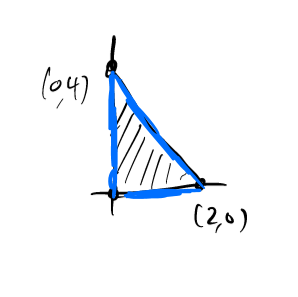
\includegraphics[width = 0.5 \textwidth]{./op1.png}
  \end{center} }
Much like the optimization problems of
single variable calculus, we need to first consider
where the possible maxima/minima could be.
\begin{itemize}
  \item Critical Points
  \item (new!) Boundary Points

\end{itemize}
Let us start by finding the critical points of
$f(x,y)$.
Recall that $f(x,y)$ is equal to
\begin{equation} \label{eq2}
f(x,y) = xy
\end{equation}
Whenever we worked with single variable calculus,
we evaluated the derivative of the function.
However, since we are now working with a
\textbf{multivariable function}, we now accordingly
work with \textbf{gradients}.
\[ \Rightarrow \nabla f = (\frac{\partial f}{\partial x}, \frac{\partial f}{\partial y} )\]
\[ \Rightarrow \nabla f = (\frac{\partial}{\partial x} (xy),
  \frac{\partial}{\partial y} (xy) ) \]
\[ \Rightarrow \partial f = \left( y, x \right)\]
Now, much like how we evaluated the critical points
by letting the derivative of a single variable function
$ f $ equal to 0, we now let the \textbf{gradient vector} equal the \textbf{zero vector}.
\[ \Rightarrow \partial f = \left( y,x \right) = (0,0) \]
\[ \Rightarrow y = 0, x = 0 \]
Our critical point is at $ y = 0, x = 0$ or at the
point $ (0,0) $.
\nt{Remember, we have ot make sure that our critical
  point is actually \textit{inside} of the
  boundaries, much like how it is supposed to be
  inside of the interval. }
Now that we have the \textbf{critical points} of
the function $ f(x,y)$, we now have to find
the \textbf{boundary points} of $ f(x,y)$
\begin{itemize}
  \item The Extreme Value Theorem for Multivariable
        Functions states that a maxima/minima
        of a function can occur at either
        the critical points or the boundary points
        of a function. We are essentially equating
        the boundary points to the \textbf{endpoints}.
\end{itemize}
But how do we actually find the ``boundary points''?
\begin{center}
  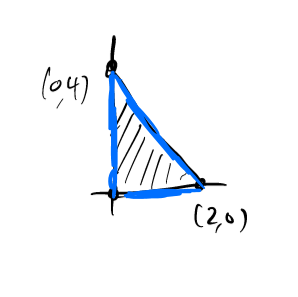
\includegraphics[width = 0.5 \textwidth]{./op1.png}
\end{center}

When we look at the graph, we observe that the
triangle is bounded by the three points $ (0,0), (0,4),
(2,0)$, so we can define our boundaries by finding
the equations of the lines that contains these boundaries. We will from here on out
refer to these boundaries interchangeably with
the term \textbf{pieces}. \\

The piece from $ (0,4)$ to $(2,0)$ is
bounded by on the interval $ 0 \le x \le 2$
on the line $ y = -2x + 4 $. \\

The piece from $ (0,0) $ to $ (2,0)$ is
bounded on the interval $ 0 \le x \le 2 $
and is given by the function $ y = 0$. \\

The piece from $ (0,4) $ to $ (0,0)$ is
bounded oin the interval $ 0 \le y \le 4 $ and
is given by the function $ x = 0 $.

\begin{center}
  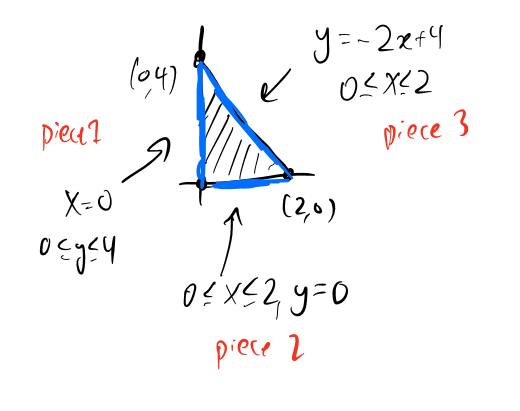
\includegraphics[width = 0.5 \textwidth]{op2.png}
\end{center}

Now, as we evaluated the function $ f$ at its
critical points $ x $ in single variable calculus,
in multivariable calculus, we now evaluate the
multivariable function $ f(x,y)$ at its
critical points as well as its boundary points.

\par For piece 1:
\[ x = 0, 0 \le y \le 4 \]
\[ \Rightarrow f(0,y) = xy \Rightarrow (0)y = 0 \]
\par For piece 2:
\[ y = 0, 0 \le x \le 2 \]
\[ \Rightarrow f(x,0) = xy = x(0) = 0 \]
\par For piece 3:
\[ y = -2x + 4, 0 \le x \le 2 \]
\[ f(x, -2x+4) = xy \Rightarrow x(-2x+4) \]
\nt{We now have a single variable equation!
  Since the values of the boundary points on this
  line have different values, we must
  find the maxima/minima \textit{of this boundary.} We
  just evaluate this equation the same exact
  way we would evaluate the maxima/minima of a
  single varialbe expression. We must derive this equation
  then let it equal 0.
}
\[ \Rightarrow g(x) = -2x^{2} + 4x = 0, x \in [0,2]\]
\[ \Rightarrow g'(x) = -4x + 4 = 0 \]
\[ \Rightarrow -4x = -4 \]
\[ \Rightarrow x = 1 \]
The critical points of $ g(x) = -2x^{2} + 4x $ are
$ x \in \{0, 1, 2\}$. So, now we must evaluate
the critical values of this boundary line $ g(x)$.

\par For $x=0$ of the boundary line $ g(x)$,
\[ g(0) = 0 \]
\par For $x=1$ of the boundayr line $ g(x)$,
\[ g(1) = -2 + 4 = 2 \]
\par For $ x=2$ of the boundary line $ g(x)$,
\[ g(2) = 0 \]

We observe that the maximum of the boundary
line $ g(x) $ is $2$ at $ x = 1 $, while
the minimum is $ 0$ at $x = 0,2 $.
\\
\par THis means that for the third piece,
the minimum occurs at $ (0,4)$ (which
is the minima of $g(x)$, $ x = 0$ in
the original function $ f(x,y)$) as well as
$ (2,0)$ (which is the minima of $ g(x)$, $ x = 2$
in the original function $ f(x,y)$). The maxiama
of piece 3 is $g(1) = -2(1) + 4(1) = 2 $, which
is $(1,2)$.

\par Now, we can assess all of the points we
have assembled from our critical values
as well as our boundary points and determine
where the maxima and minima are of our funciton.
\begin{itemize}
  \item We know that the value of $f(x,y)$ is
        0 for the first piece as well as the
        second piece, since the first piece is
        $ f(0, y) \forall 0 \le y \le 4$ and
        the second piece is $ f(x, 0) \forall
        0 \le x \le 2 $.
\end{itemize}
Let us now evaluate the boundary point $ (1, 2)$.
\[ f(x,y) = xy \Rightarrow (1)(2) = 2 \]
The global maximum of $ f(x,y)$ is $z =2$, which is
at $ (1,2)$.

\par Congrats, we just solved our first multivariable
optimization problem! Here's more to come in the
future\dots Let us now recap what exactly we did
as well as the general strategy for evaluating
multivarialbe optimizatoin problems.

\begin{enumerate}
  \item First, we found the critical points
        of our multivariable functoin $ f(x,y)$ by
        evaluating for the \textbf{gradient vector}.
        Whereas we had to let the derivative
        of our functoin equal 0 in single variable
        calculus, we let our \textbf{gradient vector}
        equal to the \textbf{zero vector}. We
        evaluate this to get the xy-coordinates
        of our critical points.
  \item Now, we can evaluate these critical points
        and find the corresponding $ z $ values.
  \item After evaluating the critical points
        as well as their values, we now find
        the \textbf{boundary points} by creating
        \textbf{pieces} from the constraints of
        the problem. In this case, we found
        lines that created the triangle we were looking
        for.
  \item With these boundary lines, again, we
        want to evaluate the values of the functoin
        along hte points of these boundary lines.
        This might be very easy, as they might just
        be zero. However, oftentimes, we will
        have more complex boundaries.
        \begin{itemize}
          \item With more complex boundaries, we
                will get a piece that has
                different values along its points.
                From this, we have to find
                the maxima and minima of this boundary
                line. By this point, we should
                have a single varialbe function,
                so we can just find the
                maxima/minima of this function
                using the tactics we already know.
          \item With these maxima and minima,
                we can then \textbf{plug
                the maxima and minima of these pieces
                into the original multivariable
                function} and we can then discern
                there value in relation to the
                prevoius boundary points and critical
                values.
        \end{itemize}
  \item At this point, we should now have
        all of the values of the most important parts
        of the function. We can now just compare
        these values and discern what the maxima and
        minima are of the general funciton.


\end{enumerate}

\section{Philosophy of Optimization}
Are we always going to be guarenteed
an answer with these problems?
\begin{itemize}
  \item Well, it's complicated. If the function is
        not closed (meaning that there aren't
        any endpoints), then it is possible
        that there aren't any maxima or minima.
        Furtheremore, if hte function wasn't
        continuous, then there also might not
        be any maxima or minima.
  \item The general criteria for achieving
        an ansewr from an optimization problem
        is as follows: we must have a \textbf{closed},
        \textbf{bounded}, and \textbf{continuous} function.
\end{itemize}

Let us try another example now

\ex{Slightly Harder Example + Introducing Parameterization}{Find the absolute extrema of
  \[f(x,y) = x^{2} + xy+y^{2} -6y
  \]
  on the region $ -3 \le x \le 3 $, $ 0 \le y \le 5 $.

\begin{center}
  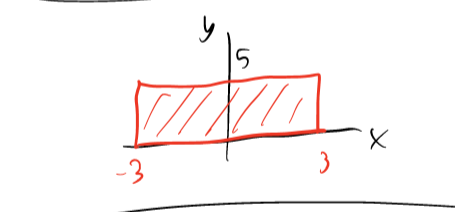
\includegraphics[width = 0.5 \textwidth]{./op3.png}
\end{center}
}
/sl Our intution reminds us that, in essence,
we must locate all the possible locations that
the extrema can occur (the critical points and the
boundary points), and then just evaluate the value
of the function at these boundary points.

\chapter{14.8: Lagrange Multipliers}
\section{Reminders}
\subsection{MATH\_226}
\begin{itemize}
  \item written homework due friday
  \item midterm in 14 days


\end{itemize}

\subsection{MATH\_230}
\begin{itemize}
  \item written homework due tonight
  \item extrema and saddle points mylab due thursday
  \item midterm in 13 days
\end{itemize}



\section{Objectives}
\begin{itemize}
  \item Derive the intuition and understanding behind Lagrange Multipliers
  \item Be able to apply Lagrange Multipliers to any problem
\end{itemize}

\section{Motivation}
In the previous section, \textbf{Optimization}, we discussed different ways to evaluate the extrema of a surface.
\begin{itemize}
  \item We realized that we have to not only consider the critical points, but also the \textit{boundary points} of the level curves of a multivariable function

\end{itemize}
However, what if we wanted to anazlye the extrema of a surface on a very \textit{specific subset} of the surface. Sure, we could always just pull out our optimization techniques, analyze the boundary points, make pieces, and evaluate the critical points within these boundaries, however, this isn't very \textit{efficient}. Instead, let us examine a new method of analyzing extrema within a function using a technique called \textit{Lagrange Multipliers}.

\section{Introduction: Constrained Maxima and Minima}
In order to begin, let us consider a trivial example in which we analyze where a minimum can be in a \textit{constrained subset} of a graph, as well as strategies to actually finding this minimum.
\ex{Finding Extrema within a Constrained Subset}{Find the point $(x,y,z)$ on the plane $ 2x + y - z = 0 $
  that is \textit{closest to the origin}. }
\sol The problem is essentially asking us to \textit{minimize the distance from the origin to a point $\overrightarrow{OP}$, so we know that we
  are basically trying to find the smallest possible
  point $ P$ that satisfies}

\begin{equation}
  \overrightarrow{OP}= \sqrt{(x-0)^{2}+(y-0)^{2}+(z-0)^{2}} \\
  &= \sqrt{x^{2}+y^{2}+z^{2}}

\end{align}

but also satisfies the fact that the point $ (x,y,z)$ exists on the plane
\begin{align}
  &= 2x+y-z + 5 =0
\end{align}

What we can do here, is that we can put the equation \textit{in terms of z}.
\begin{align*} \label{}
  &z = 2x + y +5
\end{align*}

which means that we can let $ f $ just be
\begin{align}
  &= h(x,y) = f(x, y, 2x+y+5) \\
  &= x^{2} + y^{2} + (2x+y+5)^{2}
\end{align}

\section{General Method of Lagrange Multipliers}
The main equation that we will utlize with Lagrange Multipliers is
\[ \nabla f(P) = \lambda \nabla g(P)\]




\chapter{14.8: Lagrange Multipliers (Part 2)}
\section{Reminders}
\section{Objectives}
\section{Motivation}
\end{sloppypar}
\end{document}
